\section{Dijkstra Algorithm}

\begin{frame}{Dijkstra Algorithm}{Shortest Path without Computer}
  \begin{itemize}
    \item
      Wanted: Shortest path from M to all other points
    \item
      Place pearls on crossings and clamp strings between them
  \end{itemize}
  \begin{figure}
    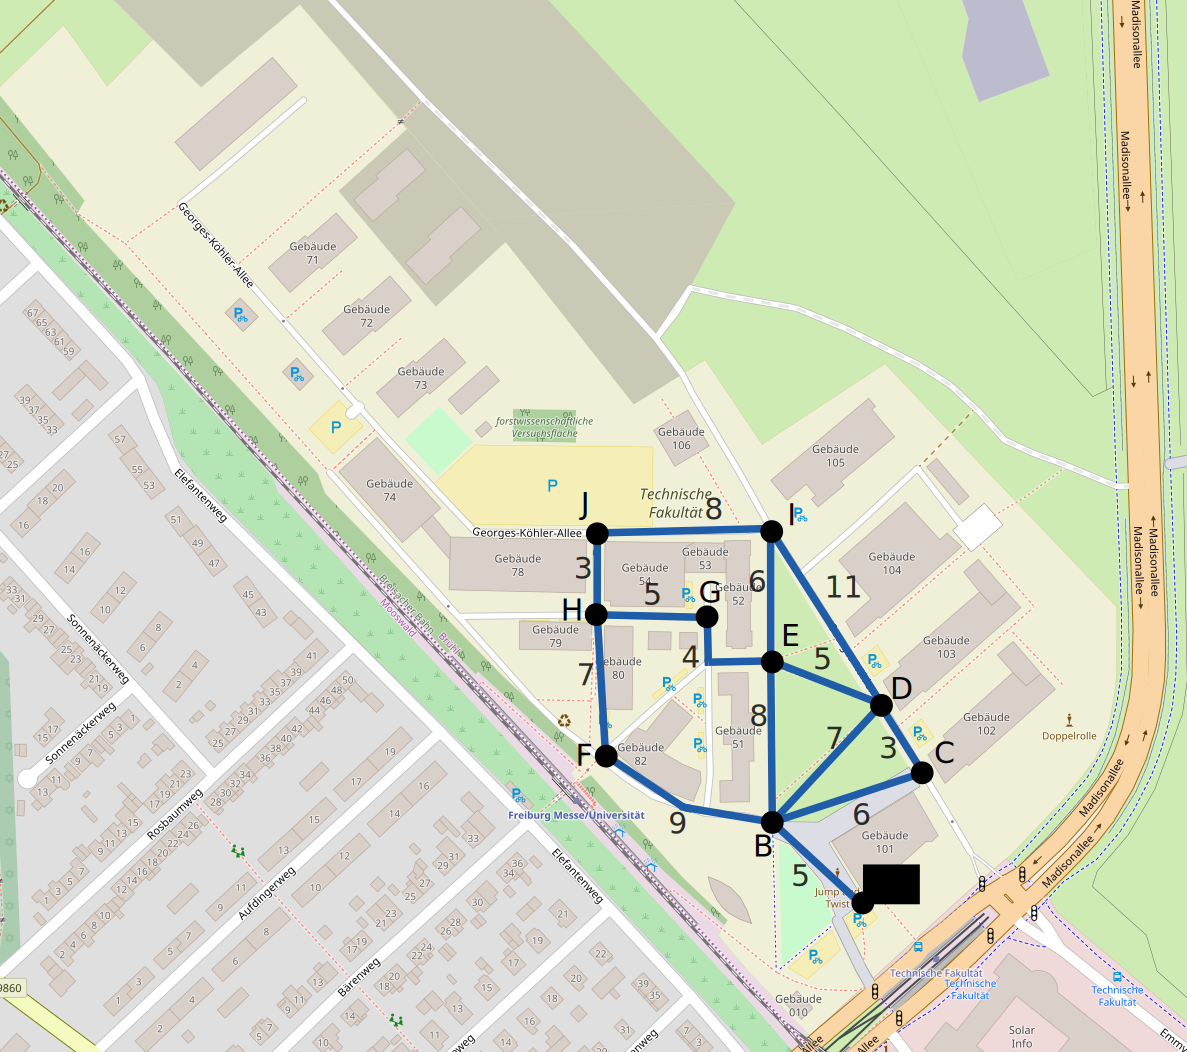
\includegraphics[width=0.45\linewidth]{Images/Dijkstra/DijkstraMapTF.png}
  \end{figure}
\end{frame}

%-------------------------------------------------------------------------------

\begin{frame}{Dijkstra Algorithm}{Shortest Path without Computer}
  \vspace{-1.5em}
  \begin{columns}
    \begin{column}{0.5\linewidth}
      \begin{figure}[!t]
        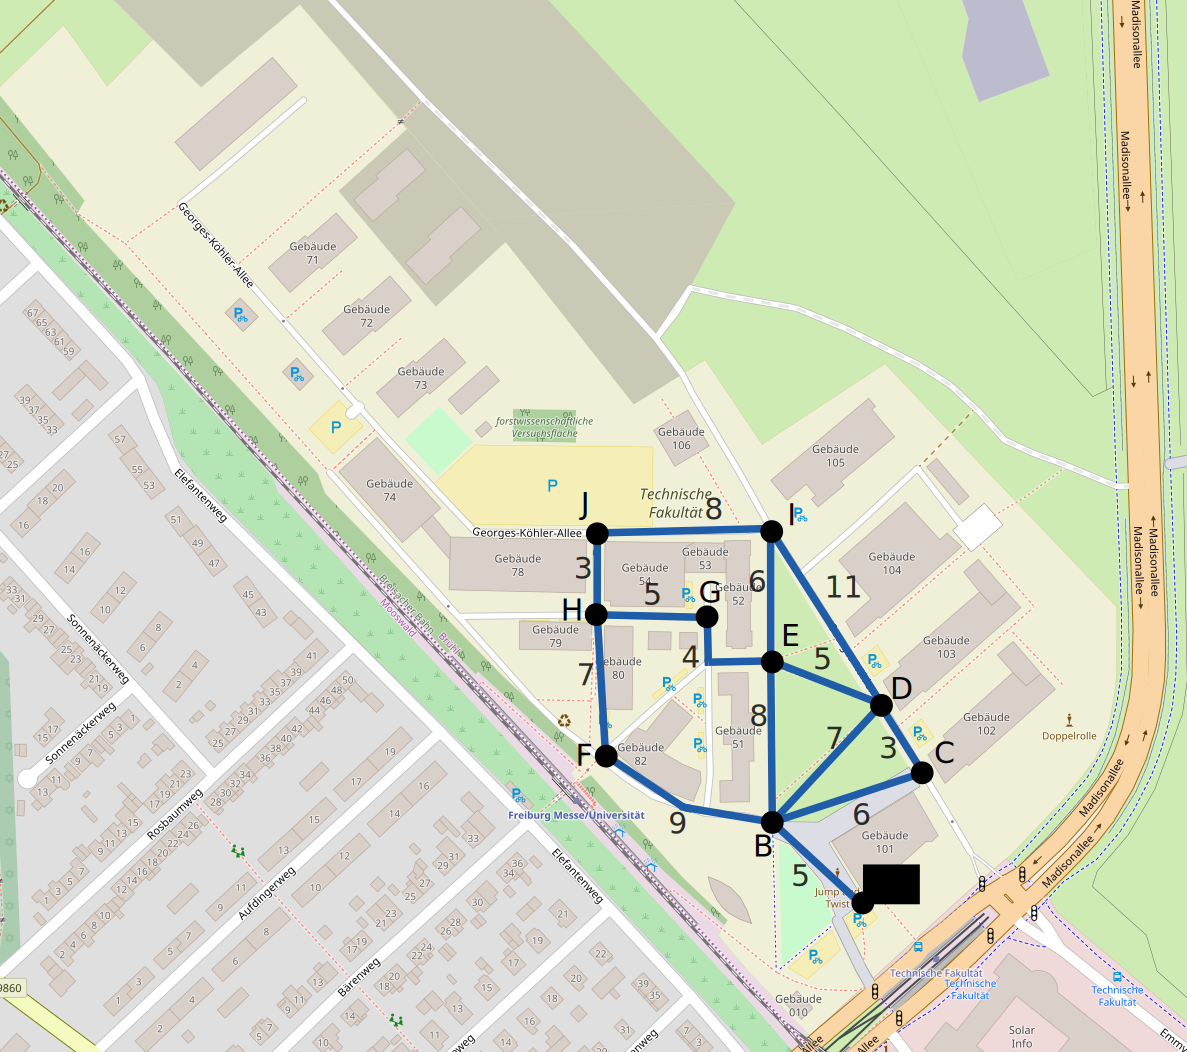
\includegraphics[width=0.6\linewidth]
          {Images/Dijkstra/DijkstraMapTF.png}
          \caption{Based on OpenStreetMaps; CC BY-SA 2.0}
      \end{figure}
      \vspace{-1.5em}
      \begin{itemize}
        \item
          Take the net and pull it slowly upwards until fully lifted
      \end{itemize}
    \end{column}
    \begin{column}{0.5\linewidth}
      \begin{figure}[!t]
        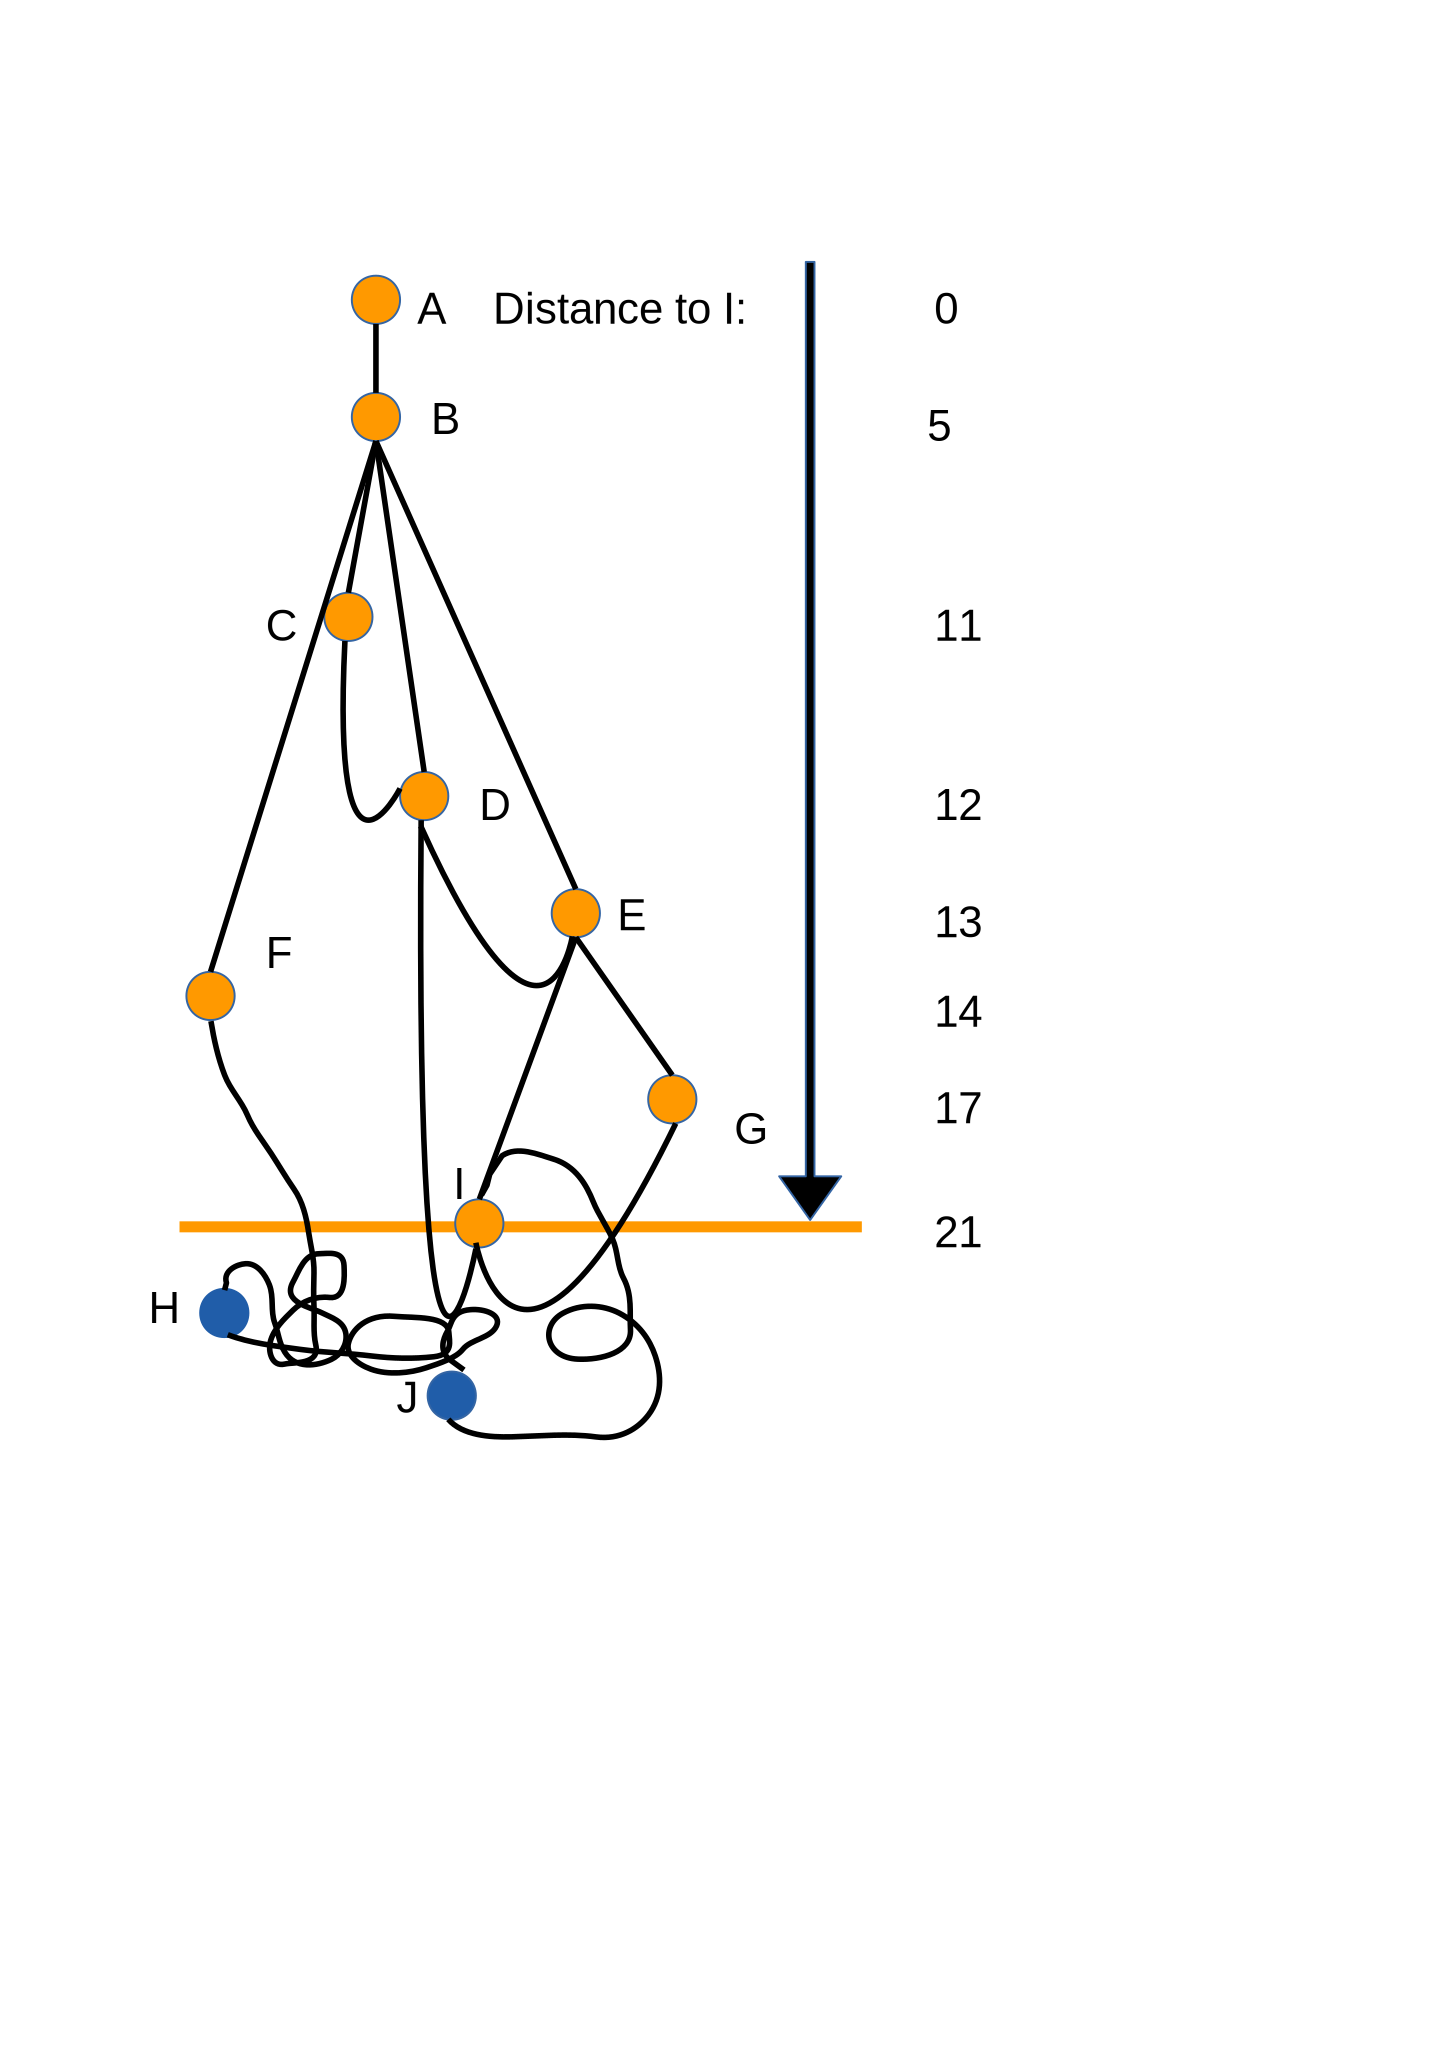
\includegraphics[width=0.7\linewidth]
          {Images/Dijkstra/DijkstraTreeTF.pdf}
        \vspace{-0.5em}
      \end{figure}
      \begin{itemize}
        \item
          Each node (pearl) now has a specific height
        \item
          The distance to M is exactly the {\color{MainA}shortest path}
        \end{itemize}
    \end{column}
  \end{columns}
\end{frame}

%-------------------------------------------------------------------------------

\begin{frame}{Dijkstra Algorithm}{Shortest Path}
  \vspace{-1.5em}
  \begin{figure}
    \begin{adjustbox}{width=0.75\linewidth}
      \begin{tikzpicture}[
  vertex/.style={
    circle,
    draw=Mittel-Blau,
    color=Mittel-Blau,
    fill=Hell-Blau,
    inner sep=0em,
    minimum size=1.75em,
    line width=0.1em,
    font=\large,
    solid
  }, vertex_shadow/.style={
    vertex,
    draw=black,
    color=black,
    fill=white,
    dotted
  }, edge/.style={
    draw=Mittel-Gruen,
    line width=0.2em
  }, edge_arrow/.style={
    edge,
    ->
  }, edge_label/.style={
    sloped,
    anchor=south,
    auto=false
  }
]%
% Draw vertices
\draw (9.0, 0.0) node[vertex] (end) {$t$};
\draw[edge_arrow, dashdotted]
  (0.0, 0.0) .. controls (3.0, 1.5) and (6.0, 0.0) .. (end.west)
  node[vertex, pos=0.0] {$s$}
  node[vertex, pos=0.2] {$u_1$}
  node[vertex_shadow, pos=0.4] {}
  node[vertex, pos=0.6] {$u_2$}
  node[vertex_shadow, pos=0.8] {}
  node[pos=0.5, above] {\color{Mittel-Gruen}$r$};
\end{tikzpicture}%
    \end{adjustbox}
    \label{fig:dijkstra:shortest_path_introduction}
    \caption{Shortest path from {\color{MainA}$s$} to
    {\color{MainA}$t$}}
  \end{figure}
  \vspace{-1.5em}
  \begin{itemize}
    \item
      Let {\color{MainB}$r$} be the shortest path from
      {\color{MainA}$s$} to {\color{MainA}$t$}
    \item
      For each node {\color{MainA}$u$} on path {\color{MainB}$r$}
      the path from {\color{MainA}$u$} to {\color{MainA}$t$} is
      the shortest path
  \end{itemize}
  \textbf{Proof:}
  \begin{itemize}
    \item
      If there was a shorter path from {\color{MainA}$s$} to
      {\color{MainA}$u$} then we could choose this path to get faster to
      {\color{MainA}$t$}
    \item
      Then {\color{MainB}$r$} would not be the shortest path
  \end{itemize}
\end{frame}

%-------------------------------------------------------------------------------

\begin{frame}{Dijkstra Algorithm}{Shortest Path}
  \vspace{-1.5em}
  \begin{figure}
    \begin{adjustbox}{width=0.75\linewidth}
      \begin{tikzpicture}[
  vertex/.style={
    circle,
    draw=Mittel-Blau,
    color=Mittel-Blau,
    fill=Hell-Blau,
    inner sep=0em,
    minimum size=1.75em,
    line width=0.1em,
    font=\large,
    solid
  }, vertex_shadow/.style={
    vertex,
    draw=black,
    color=black,
    fill=white,
    dotted
  }, edge/.style={
    draw=Mittel-Gruen,
    line width=0.2em
  }, edge_arrow/.style={
    edge,
    ->
  }, edge_label/.style={
    sloped,
    anchor=south,
    auto=false
  }
]%
% Draw vertices
\draw (9.0, 0.0) node[vertex] (end) {$t$};
\draw[edge_arrow, dashdotted]
  (0.0, 0.0) .. controls (3.0, 1.5) and (6.0, 0.0) .. (end.west)
  node[vertex, pos=0.0] {$s$}
  node[vertex, pos=0.2] {$u_1$}
  node[vertex_shadow, pos=0.4] {}
  node[vertex, pos=0.6] {$u_2$}
  node[vertex_shadow, pos=0.8] {}
  node[pos=0.5, above] {\color{Mittel-Gruen}$r$};
\end{tikzpicture}%
    \end{adjustbox}
    \label{fig:dijkstra:shortest_path_introduction_re}
    \caption{Shortest path from {\color{MainA}$s$} to
      {\color{MainA}$t$}}
  \end{figure}
  \vspace{-1.5em}
  \begin{itemize}
    \item
      This is also correct for all sub paths on {\color{MainB}$r$}
    \item
      If the shortest path from {\color{MainA}$s$} to
      {\color{MainA}$t$} passes {\color{MainA}$u_1$} and
      {\color{MainA}$u_2$} then the sub path
      $({\color{MainA}u_1}, {\color{MainA}u_2})$
      is the shortest path from {\color{MainA}$u_1$} to
      {\color{MainA}$u_2$}
  \end{itemize}
\end{frame}

%-------------------------------------------------------------------------------

\begin{frame}{Dijkstra Algorithm}{Shortest Path}
  \begin{figure}%
    \begin{adjustbox}{width=0.75\linewidth}%
      \begin{tikzpicture}[
  vertex/.style={
    circle,
    draw=Mittel-Blau,
    color=Mittel-Blau,
    fill=Hell-Blau,
    inner sep=0em,
    minimum size=1.75em,
    line width=0.1em,
    font=\large,
    solid
  }, vertex_shadow/.style={
    vertex,
    draw=black,
    color=black,
    fill=white,
    dotted
  }, edge/.style={
    draw=Mittel-Gruen,
    line width=0.2em
  }, edge_arrow/.style={
    edge,
    ->
  }, edge_label/.style={
    sloped,
    midway,
    color=Mittel-Gruen
  }
]%
% Draw vertices
\draw (-2.0, 0.0) node[vertex] (start) {$s$};
\draw (10.0, 0.0) node[vertex] (end) {$t$};

\draw[edge_arrow] (7.5, 1.5) node[vertex] (v1) {$v_1$} to
  node[edge_label, above] {16} (end);
\draw[edge_arrow] (7.5, 0.0) node[vertex] (v2) {$v_2$} to
  node[edge_label, above] {3} (end);
\draw[edge_arrow] (7.5, -1.5) node[vertex] (v3) {$v_3$} to
  node[edge_label, above] {2} (end);

\draw[edge_arrow, dashdotted]
  (start) .. controls (3.0, 2.5) and (6.0, 1.0) .. (v1.west)
  node[vertex_shadow, pos=0.2] {}
  node[vertex_shadow, pos=0.4] {}
  node[vertex_shadow, pos=0.6] {}
  node[vertex_shadow, pos=0.8] {}
  node[edge_label, pos=0.5, above] {22};
\draw[edge_arrow, dashdotted]
  (start) .. controls (3.0, -1.0) and (6.0, 0.0) .. (v2.west)
  node[vertex_shadow, pos=0.25] {}
  node[vertex_shadow, pos=0.4] {}
  node[vertex_shadow, pos=0.6] {}
  node[edge_label, pos=0.5, above] {34};
\draw[edge_arrow, dashdotted]
  (start) .. controls (3.0, -3.0) and (6.0, -1.5) .. (v3.west)
  node[vertex_shadow, pos=0.1] {}
  node[vertex_shadow, pos=0.3] {}
  node[vertex_shadow, pos=0.8] {}
  node[edge_label, pos=0.5, above] {42};
\end{tikzpicture}%%
    \end{adjustbox}%
    \vspace{-1.0em}
    \label{fig:dijkstra:shortest_paths_introduction}%
    \caption{Shortest paths from {\color{MainA}$s$} to
      {\color{MainA}$t$}}
  \end{figure}
  \vspace{-1.0em}
  \begin{itemize}
    \item
      If we know the shortest path form {\color{MainA}$s$}
      to the preceding nodes of {\color{MainA}$t$}
      \begin{math}
        (
          {\color{MainA}v_1},
          {\color{MainA}v_2},
          {\color{MainA}v_3}
        )
       \end{math}
       we can determine the shortest path to {\color{MainA}$t$}
   \end{itemize}
\end{frame}

%-------------------------------------------------------------------------------

\begin{frame}{Dijkstra Algorithm}{Shortest Path}
  \textbf{Idea:}
  \begin{itemize}
    \item
      Attach the cost of the shortest path to each node
    \item
      Let the information travel over the edges (message passing)
    \item
      In which order should we process the nodes?
  \end{itemize}
\end{frame}

%-------------------------------------------------------------------------------

\begin{frame}{Dijkstra Algorithm}
  \begin{columns}
    \begin{column}{0.6\linewidth}
      \textbf{Inventor:}
      \begin{itemize}
        \item
          Edsger Dijkstra (1930 - 2002)
        \item
          Computer scientist from Netherlands
        \item
          Won Turing-Award as one of few Europeans for his studies of 
          structured programming
        \item
          Invented the Dijkstra-Algorithm in 1959
      \end{itemize}
    \end{column}
    \begin{column}{0.4\linewidth}
      \begin{figure}
        \includegraphics[width=0.75\linewidth]
          {Images/Dijkstra/Edsger_Wybe_Dijkstra.jpg}
        \caption{Portrait \copyright\; Hamilton Richards - manuscripts of
          Edsger W. Dijkstra, University Texas at Austin}
        \label{fig:dijkstra:portrait}
      \end{figure}
    \end{column}
  \end{columns}
\end{frame}

%-------------------------------------------------------------------------------

\begin{frame}{Dijkstra Algorithm}
  \vspace{-1.5em}
  \begin{columns}
    \begin{column}{0.55\linewidth}
      \textbf{Example:}
      \begin{itemize}
        \item
          Lift pearl {\color{MainA}$A$} a little bit
        \item
          Connection to pearl {\color{MainA}$B$} is hanging in the air
        \item
          Lift further until pearl {\color{MainA}$B$} starts to lift at
          $\SI{5}{m}$
        \item
          The shortest path to {\color{MainA}$B$} is now known
        \item
          Lift further: The wires from {\color{MainA}$C$},
          {\color{MainA}$D$}, {\color{MainA}$E$} and {\color{MainA}$F$}
          are now in the air
        \item
          One of the pearls {\color{MainA}$C$}, {\color{MainA}$D$},
          {\color{MainA}$E$} or {\color{MainA}$F$} is the next one\\
          {\color{gray}Which one?}
      \end{itemize}
    \end{column}
    \begin{column}{0.45\linewidth}
      \begin{figure}[!t]
        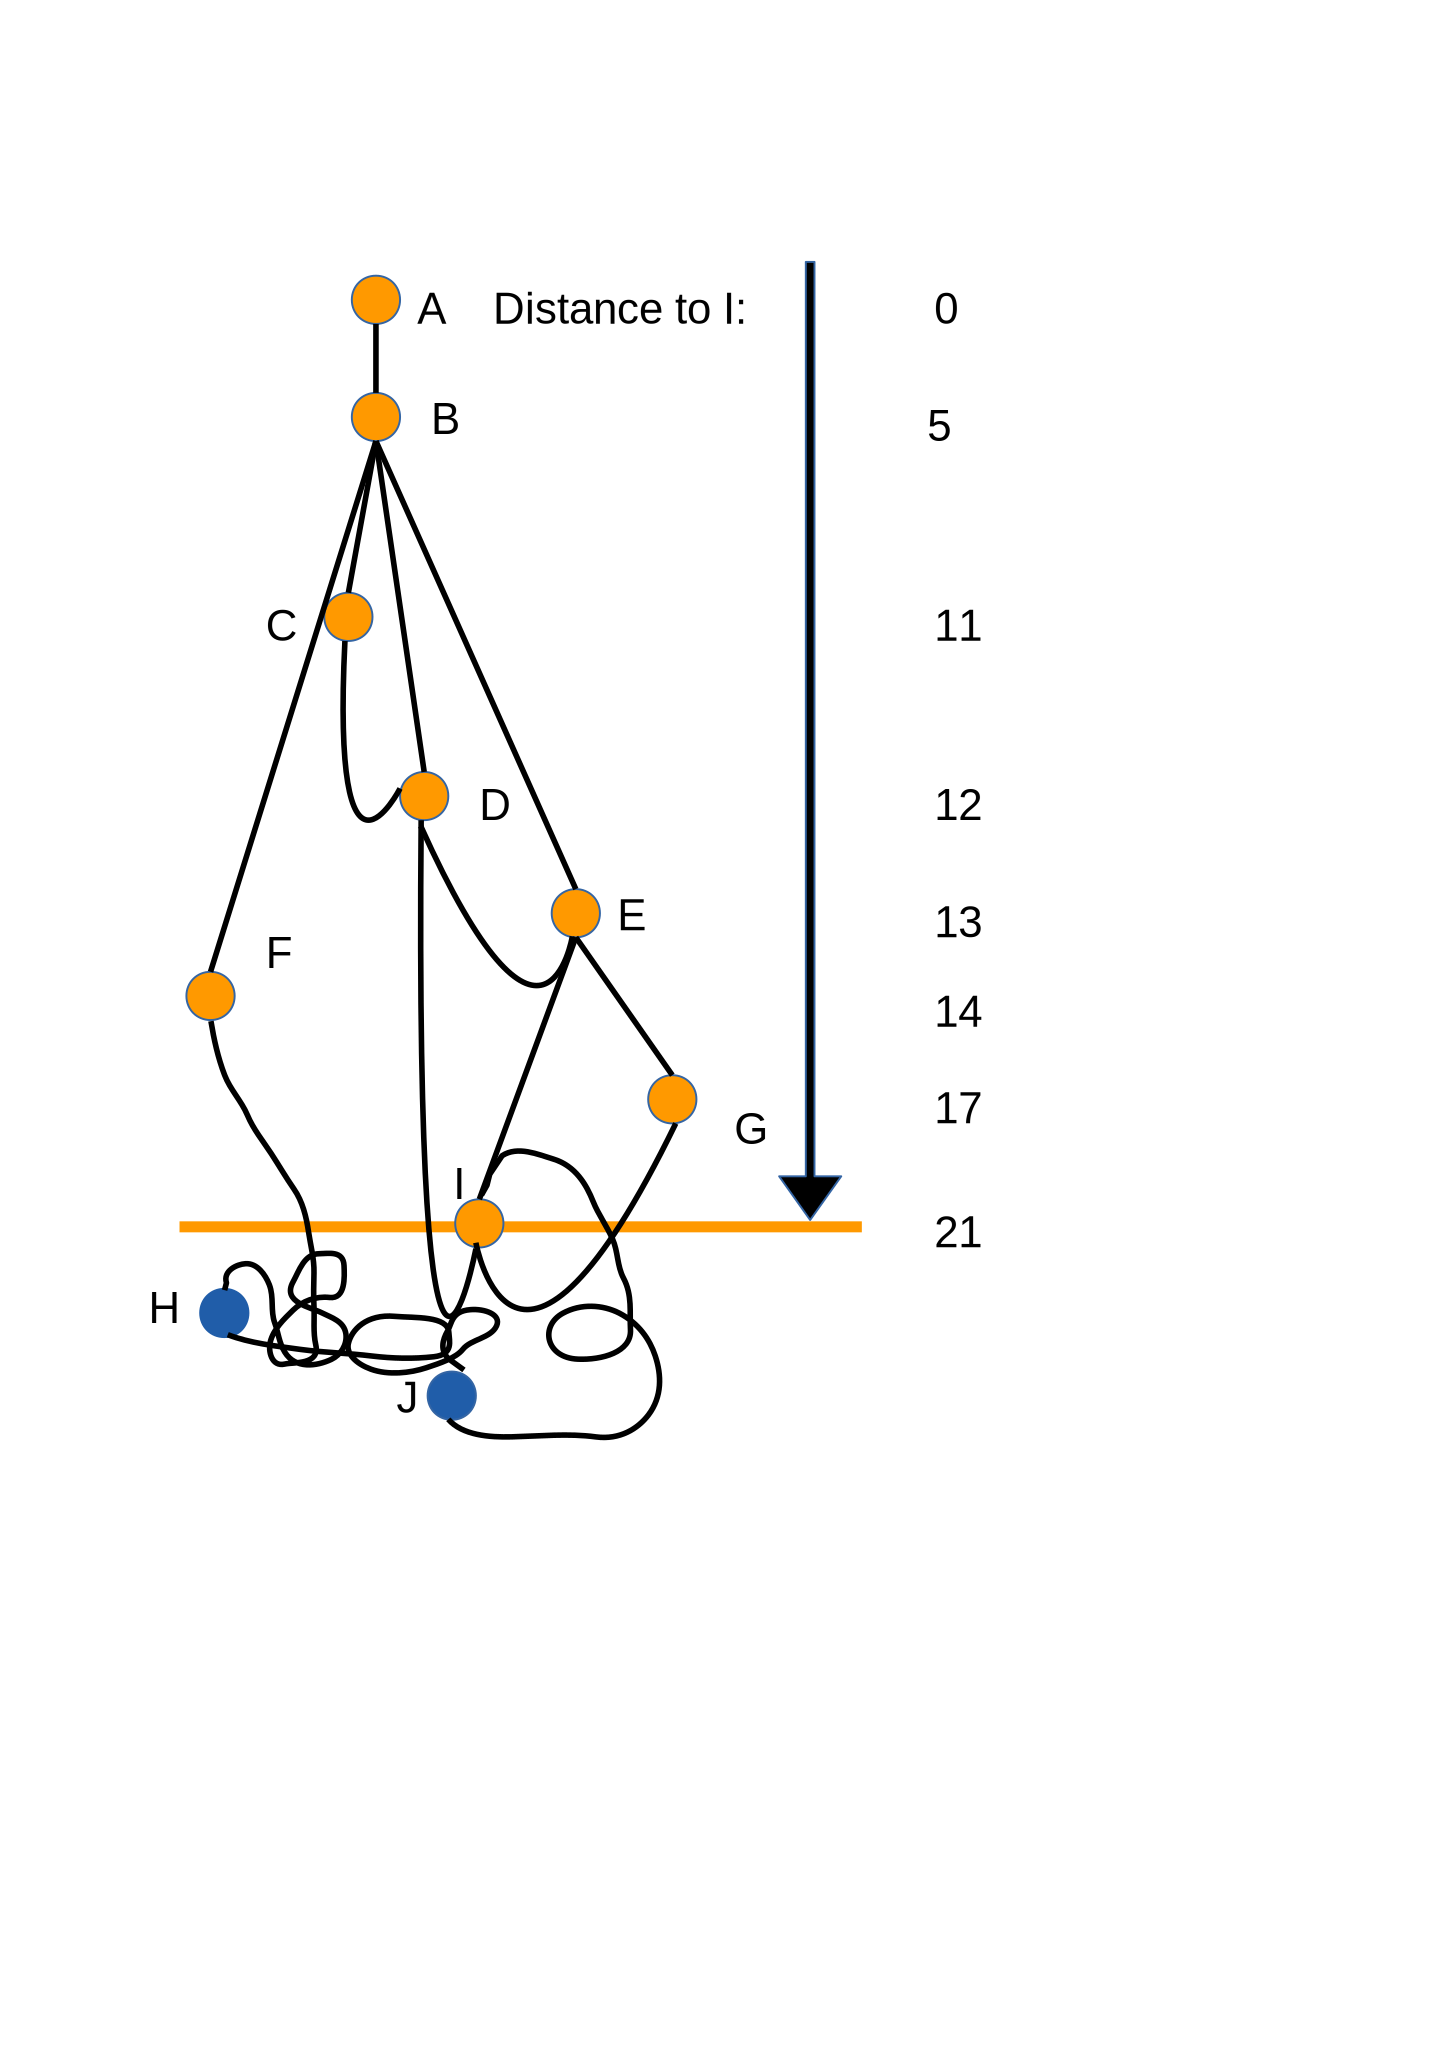
\includegraphics[width=\linewidth]
          {Images/Dijkstra/DijkstraTreeTF.pdf}
      \end{figure}
    \end{column}
  \end{columns}
\end{frame}

%-------------------------------------------------------------------------------

\begin{frame}{Dijkstra Algorithm}
  \vspace{-1.5em}
  \begin{columns}
    \begin{column}{0.55\linewidth}
      \textbf{Example:}
      \begin{itemize}
        \item
          At $\SI{11}{m}$ pearl {\color{MainA}$C$} gets lifted
        \item
          The wire to {\color{MainA}$D$} is now in the air
        \item
          One of the pearls {\color{MainA}$D$}, {\color{MainA}$E$}
          and {\color{MainA}$F$} is the next one\\
          {\color{gray}Which one?}
        \item
          At $\SI{12}{m}$ pearl {\color{MainA}$D$} gets lifted\\
          $\cdots$
        \item
          {\color{gray}How to translate this into an computer algorithm?}
      \end{itemize}
    \end{column}
    \begin{column}{0.45\linewidth}
      \begin{figure}[!t]
        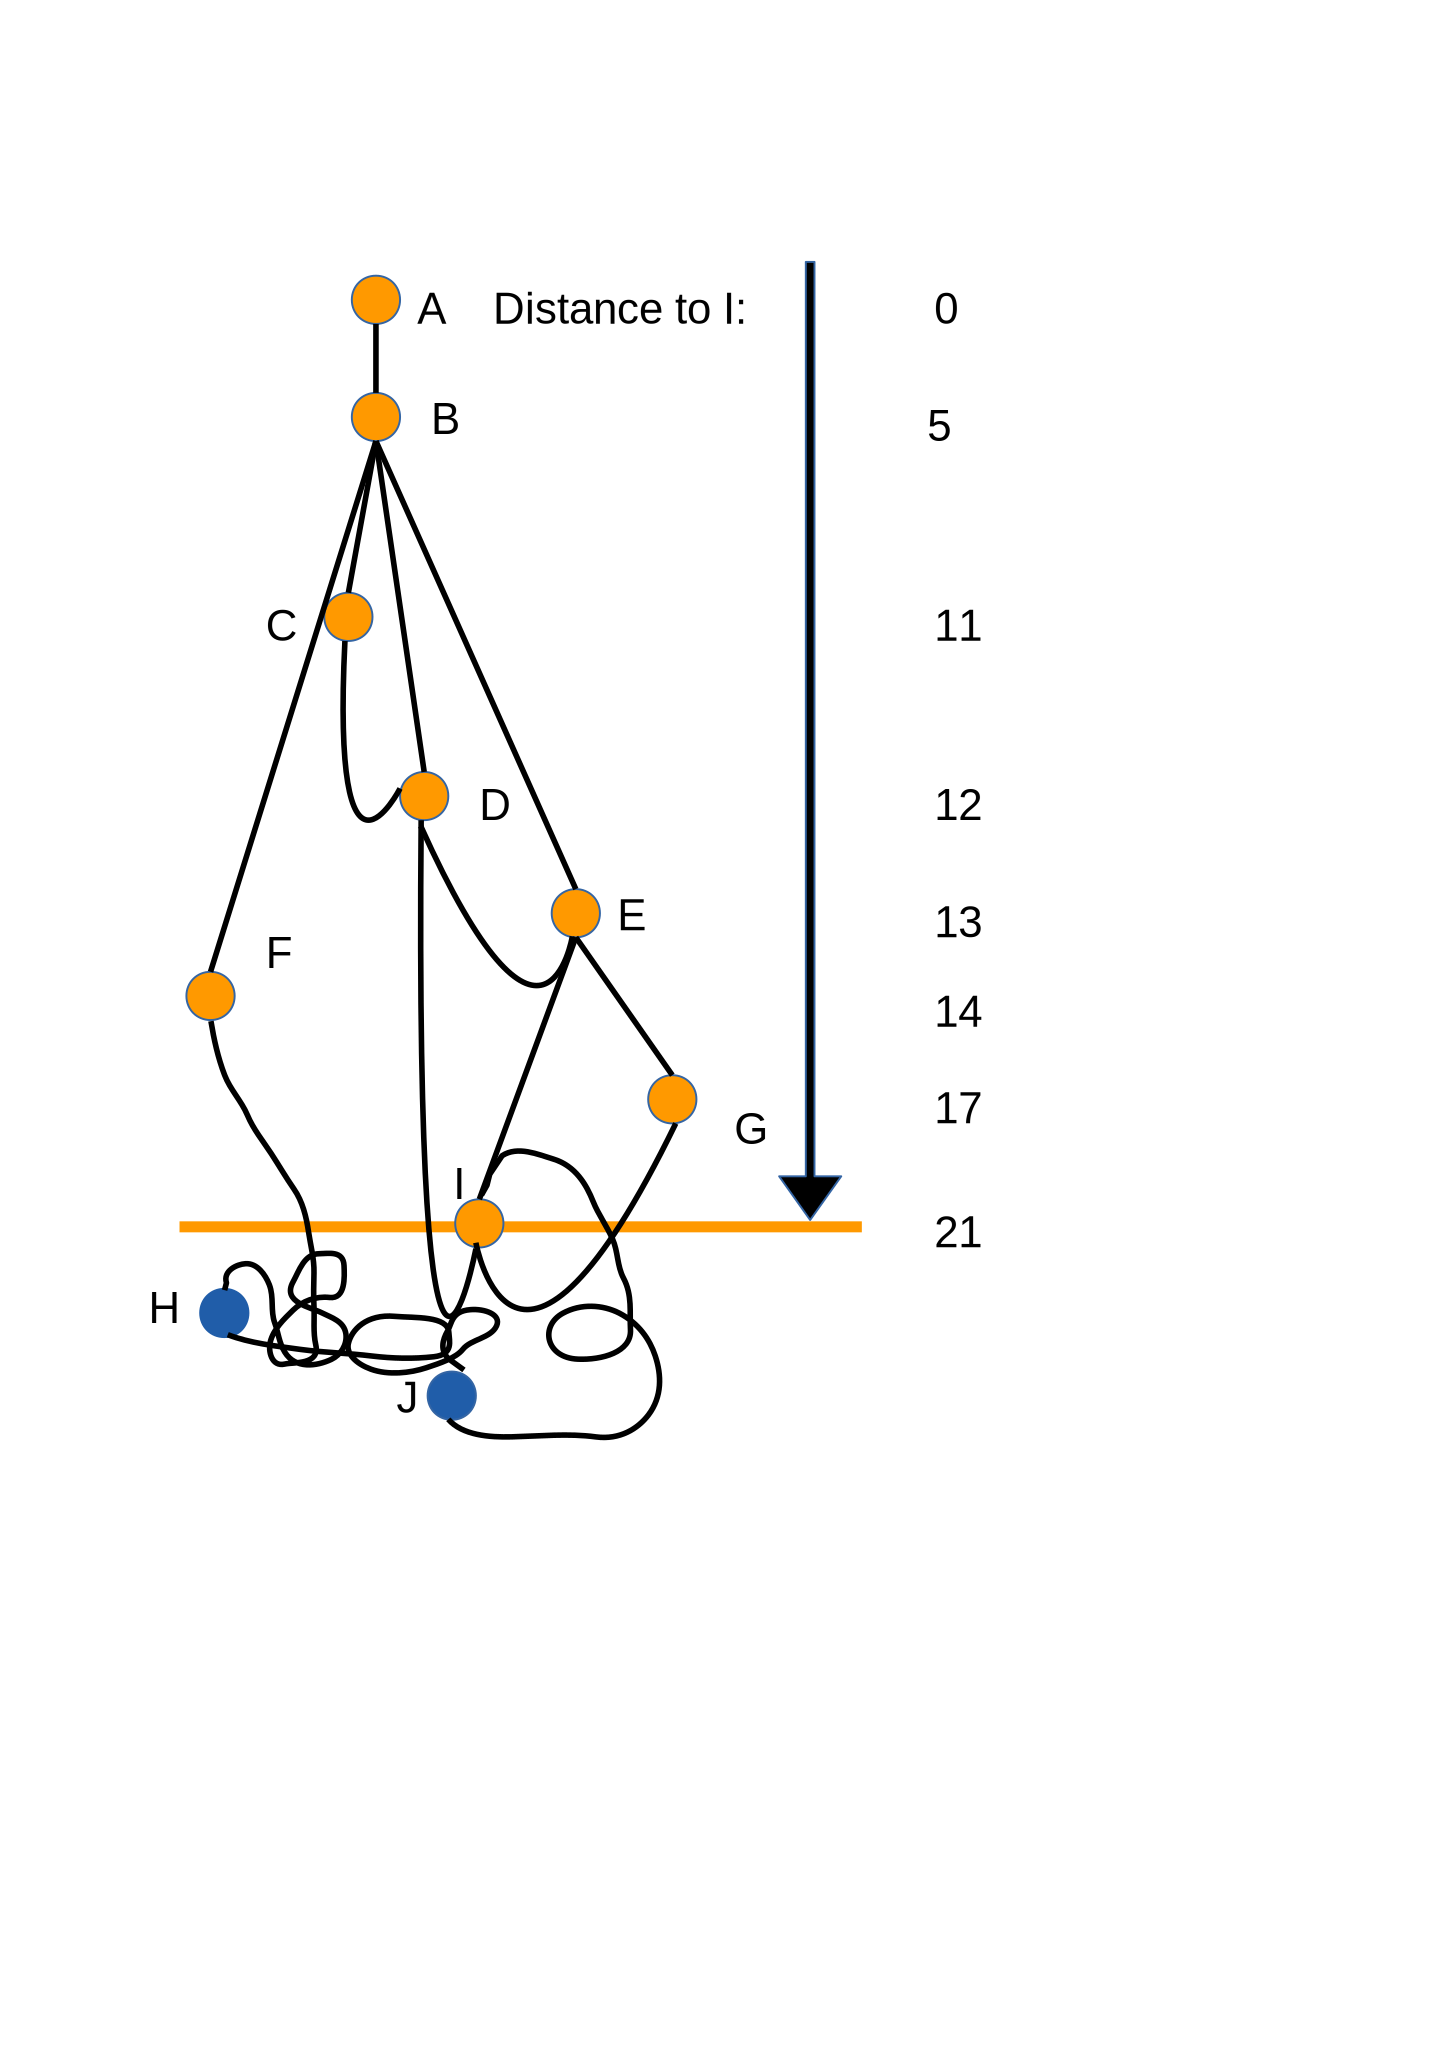
\includegraphics[width=\linewidth]
          {Images/Dijkstra/DijkstraTreeTF.pdf}
      \end{figure}
    \end{column}
  \end{columns}
\end{frame}

%-------------------------------------------------------------------------------

\begin{frame}{Dijkstra Algorithm}
  \textbf{High level description:}
  Three types of nodes
  \begin{itemize}
    \item
      {\color{MainA}Settled:}
      For node {\color{MainA}$u$} we know
      {\color{MainA}$\mathrm{dist}(s, u)$}
      \hfill
      \raisebox{-0.5em}{\begin{adjustbox}{height=1.5em}%
        \begin{tikzpicture}[
  vertex_base/.style={
    circle,
    inner sep=0em,
    minimum size=1.75em,
    line width=0.1em,
    font=\large,
    solid
  },
  vertex_settled/.style={
    vertex_base,
    draw=Mittel-Blau,
    color=Mittel-Blau,
    fill=orange!50!yellow
  }
]%
\draw (0, 0) node[vertex_settled] {42};
\end{tikzpicture}%
%
      \end{adjustbox}}\\
      {\color{gray}(Pearl example: This pearl is hanging in the air)}
      \vspace{0.5em}
    \item
      {\color{MainA}Active:}
      For node {\color{MainA}$u$} we know a tentative distance
      {\color{MainA}$\mathrm{td}(u) \geq \mathrm{dist}(s, u)$}
      (Can be optimal but doesn't have to)
      \hfill
      \raisebox{-0.5em}{\begin{adjustbox}{height=1.5em}%
        \begin{tikzpicture}[
  vertex_base/.style={
    circle,
    inner sep=0em,
    minimum size=1.75em,
    line width=0.1em,
    font=\large,
    solid
  },
  vertex_active/.style={
    vertex_base,
    draw=Mittel-Blau,
    color=Mittel-Blau,
    fill=Hell-Blau
  }
]%
\draw (0, 0) node[vertex_active] {37};
\end{tikzpicture}%
%
      \end{adjustbox}}\\
      {\color{gray}(Pearl example: This pearl is laying on the table but\\
        one connected wire is already in the air)}
        \vspace{0.5em}
    \item
      {\color{MainA}Unreached:}
      We have not reached the node yet
      \hfill
      \raisebox{-0.5em}{\begin{adjustbox}{height=1.5em}%
          \begin{tikzpicture}[
  vertex_base/.style={
    circle,
    inner sep=0em,
    minimum size=1.75em,
    line width=0.1em,
    font=\large,
    solid
  }, vertex_unreached/.style={
    vertex_base,
    draw=Mittel-Blau,
    color=Mittel-Blau,
    fill=white
  }
]%
\draw (0, 0) node[vertex_unreached] {};
\end{tikzpicture}%%
        \end{adjustbox}}\\
        {\color{gray}(Pearl example: This preal is hanging in the air)}
  \end{itemize}
\end{frame}

%-------------------------------------------------------------------------------

\begin{frame}{Dijkstra Algorithm}
  \textbf{High level description:}
  \begin{itemize}
    \item
      Each iteration take the {\color{MainA}active} node
      {\color{MainA}$u$} with the
      {\color{MainA}smallest $\mathrm{td}(u)$}\\
      {\color{gray}(The pearl getting lifted next)}
    \item
      We update the state of the node {\color{MainA}$u$} to
      {\color{MainA}settled}\\
      {\color{gray}(The pearl gets lifted)}
    \item
      We check for each {\color{MainA}neighbor $v$} of node
      {\color{MainA}$u$} if we can reach {\color{MainA}$v$} faster
      than currently possible\\
      {\color{gray}(Check all outgoing wires from this pearl:
        Activate all connected pearls, update
        tentative distance if smaller)}
    \item
      Iterate until no active nodes exist anymore
  \end{itemize}
\end{frame}

%-------------------------------------------------------------------------------

\begin{frame}{Dijkstra Algorithm}
  \vspace{-1em}
  \begin{figure}[!h]
    \begin{adjustbox}{width=\linewidth}
      \def\DijkstraReverse{0}%
      \begin{tikzpicture}[
  vertex_base/.style={
   circle,
   inner sep=0em,
   minimum size=1.75em,
   line width=0.1em,
   font=\large,
   solid
  }, vertex_active/.style={
    vertex_base,
    draw=Mittel-Blau,
    color=Mittel-Blau,
    fill=orange!50!yellow
  }, vertex_settled/.style={
    vertex_base,
    draw=Mittel-Blau,
    color=Mittel-Blau,
    fill=Hell-Blau
  }, vertex_unreached/.style={
    vertex_base,
    draw=Mittel-Blau,
    color=Mittel-Blau,
    fill=white
  }, vertex_label/.style={
    font=\large,
    color=Mittel-Blau
  }, vertex_old/.style={
    draw,
    color=gray,
    strike out,
    line width=0.1em
  }, edge/.style={
    draw=Mittel-Gruen,
    line width=0.2em
  }, edge_arrow/.style={
    edge,
    ->
  }, edge_cost/.style={
    midway,
    color=Hell-Gruen,
    font=\Large
  }, edge_highlight/.style={
    edge_arrow,
    preaction={
      draw,yellow,-,% Draw yellow without any arrow head
      double=yellow,
      double distance=2\pgflinewidth,
    }
  }
]%
% Vertex 3 old values
\only<3>{ % Value 1
  \draw ($(4, 0) + (-1em, -1em)$) node[vertex_old] {5};
}
\only<4>{ % Value 2
  \draw ($(4, 0) + (-1em, -1em)$) node[vertex_old] {4};
}

% Vertex 4 old values
\only<5>{ % Value 1
  \draw ($(4, -2.5) + (-1em, -1em)$) node[vertex_old] {10};
}

% Vertex 0
\only<1>{
  \draw (-1.0, 0.0) node[
    vertex_active,
    label={[vertex_label, shift={(-1em, -0.5em)}]above:$u_0$}
  ] (vert0) {0};
}
\only<2->{
  \draw (-1.0, 0.0) node[
    vertex_settled,
    label={[vertex_label, shift={(-1em, -0.5em)}]above:$u_0$}
  ] (vert0) {0};
}

% Vertex 1
\only<1>{
  \draw (2.5, 2.5) node[vertex_unreached] (vert1) {$u_1$};
}
\only<2>{
  \draw (2.5, 2.5) node[
    vertex_active,
    label={[vertex_label, shift={(-1em, -0.5em)}]above:$u_1$}
  ] (vert1) {1};
}
\only<3->{
  \draw (2.5, 2.5) node[
    vertex_settled,
    label={[vertex_label, shift={(-1em, -0.5em)}]above:$u_1$}
  ] (vert1) {1};
}

% Vertex 2
\only<1>{
  \draw (4.0, -2.5) node[vertex_unreached] (vert2) {$u_2$};
}
\only<2-5>{
  \draw (4.0, -2.5) node[
    vertex_active,
    label={[vertex_label, shift={(-1.5em, 0em)}]above:$u_2$}
  ] (vert2) {%
    \only<2-4>{10}%
    \only<5->{6}%
  };
}
\only<6->{
  \draw (4.0, -2.5) node[
    vertex_settled,
    label={[vertex_label, shift={(-1.5em, 0em)}]above:$u_2$}
  ] (vert2) {6};
};

% Vertex 3
\only<1>{
  \draw (4.0, 0.0) node[vertex_unreached] (vert3) {$u_3$};
}
\only<2-4>{
  \draw (4.0, 0.0) node[
    vertex_active,
    label={[vertex_label, shift={(-2em, -0.5em)}]$u_3$}
  ] (vert3) {%
    \only<2>{5}%
    \only<3>{4}%
    \only<4>{3}%
  };
}
\only<5->{
  \draw (4.0, 0.0) node[
    vertex_settled,
    label={[vertex_label, shift={(-2em, -0.5em)}]$u_3$}
  ] (vert3) {3};
}

% Vertex 4
\only<1-2>{
  \draw (5.5, 2.5) node[vertex_unreached] (vert4) {$u_4$};
}
\only<3>{
  \draw (5.5, 2.5) node[
    vertex_active,
    label={[vertex_label, shift={(1em, -0.5em)}]$u_4$}
  ] (vert4) {2};
}
\only<4->{
  \draw (5.5, 2.5) node[
    vertex_settled,
    label={[vertex_label, shift={(1em, -0.5em)}]$u_4$}
  ] (vert4) {2};
}

% Vertex 5
\only<1-3>{
  \draw (9.0, 0.0) node[vertex_unreached] (vert5) {$u_5$};
}
\only<4-6>{
  \draw (9.0, 0.0) node[
    vertex_active,
    label={[vertex_label, shift={(1em, -0.5em)}]$u_4$}
  ] (vert5) {6};
}
\only<7>{
  \draw (9.0, 0.0) node[
    vertex_settled,
    label={[vertex_label, shift={(1em, -0.5em)}]$u_4$}
  ] (vert5) {6};
}

% Edges from vertex 0
\only<1,3->{\draw[edge_arrow] (vert0) to node[edge_cost, above] {1} (vert1);}
\only<2>{\draw[edge_highlight] (vert0) to node[edge_cost, above] {1} (vert1);}

\only<1,3->{\draw[edge_arrow] (vert0) to node[edge_cost, above] {10} (vert2);}
\only<2>{\draw[edge_highlight] (vert0) to node[edge_cost, above] {10} (vert2);}

\only<1,3->{\draw[edge_arrow] (vert0) to node[edge_cost, above] {5} (vert3);}
\only<2>{\draw[edge_highlight] (vert0) to node[edge_cost, above] {5} (vert3);}

% Edges from vertex 1
\only<1-2,4->{\draw[edge_arrow] (vert1) to node[edge_cost, above] {3} (vert3);}
\only<3>{\draw[edge_highlight] (vert1) to node[edge_cost, above] {3} (vert3);}

\only<1-2,4->{\draw[edge_arrow] (vert1) to node[edge_cost, above] {1} (vert4);}
\only<3>{\draw[edge_highlight] (vert1) to node[edge_cost, above] {1} (vert4);}

% Edges from vertex 2
\only<1-5,7>{\draw[edge_arrow] (vert2) to node[edge_cost, above] {7} (vert5);}
\only<6>{\draw[edge_highlight] (vert2) to node[edge_cost, above] {7} (vert5);}

\only<6>{
  \draw[
  edge_highlight,
  bend right=15
  ] (vert2) to node[edge_cost, right] {3} (vert3);
}

% Edges from vertex 3
\only<5>{
  \draw[
    edge_highlight, bend right=15
  ] (vert3) to node[edge_cost, left] {3} (vert2);
}

% Edges from vertex 4
\only<1-3,4->{\draw[edge_arrow] (vert4) to node[edge_cost, above] {1} (vert3);}
\only<4>{\draw[edge_highlight] (vert4) to node[edge_cost, above] {1} (vert3);}

\only<1-3,4->{\draw[edge_arrow] (vert4) to node[edge_cost, above] {4} (vert5);}
\only<4>{\draw[edge_highlight] (vert4) to node[edge_cost, above] {4} (vert5);}

% Edges from vertex 5
\draw[edge_arrow] (vert5) to node[edge_cost, above] {2} (vert3);

% Overlay
\only<1-5,7>{
  \draw[
    edge_arrow,
    bend right=15
  ] (vert2) to node[edge_cost, right] {3} (vert3);
}
\only<1-4,6->{
  \draw[edge_arrow, bend right=15] (vert3) to node[edge_cost, left] {3} (vert2);
}
\end{tikzpicture}%
    \end{adjustbox}
    \vspace{-2em}
    \caption{%
      \only<1>{Start at {\color{MainA}$u_1$}}%
      \only<2>{Iteration 1}%
      \only<3>{Iteration 2}%
      \only<4>{Iteration 3}%
      \only<5>{Iteration 4}%
      \only<6>{Iteration 5}%
      \only<7>{Iteration 6}%
    }
  \end{figure}
\end{frame}

%-------------------------------------------------------------------------------

\begin{frame}{Dijkstra Algorithm}{Proof}
  \textbf{Proof:}
  \begin{itemize}
    \item
      \textbf{Assumption 1:}
      All edges have a positive length
    \item
      \textbf{Assumption 2:}
      Each node has a unique distance
      {\color{MainA}$\mathrm{dist}(s, u)$} to the start {\color{MainA}$s$}\\
      {\color{gray}(This was not the case on the previous slides)}\\[0.5em]
      This results in an easy and intuitive proof.\\
      {\color{gray}
        It is possible to show this without assumption 2.
        See references if interested}
      \vspace{1.0em}
    \item
      With assumption 2 there exists a sorting {\color{MainA}$u_1$},
      {\color{MainA}$u_2$}, $\ldots$ with that:
      \begin{displaymath}
        {\color{MainA}\mathrm{dist}(s, u_1)} <
        {\color{MainA}\mathrm{dist}(s, u_2)} <
        {\color{MainA}\mathrm{dist}(s, u_3)} <
        \ldots
      \end{displaymath}
  \end{itemize}
\end{frame}

%-------------------------------------------------------------------------------

\begin{frame}{Dijkstra Algorithm}{Proof}
  \textbf{Proof:}
  \begin{itemize}
    \item
      With \textbf{assumption 2} there exists a sorting {\color{MainA}$u_1$},
      {\color{MainA}$u_2$}, $\ldots$ with that:
      \begin{displaymath}
        {\color{MainA}\mathrm{dist}(s, u_1)} <
        {\color{MainA}\mathrm{dist}(s, u_2)} <
        {\color{MainA}\mathrm{dist}(s, u_3)} <
        \ldots
      \end{displaymath}
    \item
      We want to show that the \textit{Dijkstra} algorithm finds the shortest
      path for each node {\color{MainA}$u_i$} so that
      {\color{MainA}$\mathrm{td}(u_i) = \mathrm{dist}(s, u_i)$} holds
    \item
      Additionally we show that each node gets solved in order of the distance:
      Node {\color{MainA}$u_i$} gets solved in iteration
      {\color{MainA}$i$}
      \begin{displaymath}
        {\color{MainA}u_1},
        {\color{MainA}u_2},
        {\color{MainA}u_3},
        \ldots
      \end{displaymath}
  \end{itemize}
\end{frame}

%-------------------------------------------------------------------------------

\begin{frame}{Dijkstra Algorithm}{Proof}
  \textbf{To show:} Node {\color{MainA}$u_i$} gets solved in round
  {\color{MainA}$i$}
  \begin{enumerate}
    \item
      Node {\color{MainA}$u_i$} contains the correct distance
      ({\color{MainA}$\mathrm{td}(u_i) = \mathrm{dist}(s, u_i)$})
      and is active
    \item
      Node {\color{MainA}$u_i$} has the smallest value for
      {\color{MainA}$\mathrm{td}(u_i)$} and gets selected by the algorithm
  \end{enumerate}
  \vspace{1.0em}
  \textbf{Induction start:}
  \begin{enumerate}
    \item
      \begin{itemize}
        \item
          Only the start node {\color{MainA}$s = u_1$} is active and
          {\color{MainA}$\mathrm{td}(s) = 0$}
        \item
          Node {\color{MainA}$u_1$} gets solved and
          {\color{MainA}$\mathrm{td}(u_1) = \mathrm{dist}(s, u_1) = 0$}
      \end{itemize}
    \item
      Only the start node {\color{MainA}$u_1$} is active
  \end{enumerate}
\end{frame}

%-------------------------------------------------------------------------------

\begin{frame}{Dijkstra Algorithm}{Proof}
  \textbf{Induction step:} {\color{MainA}$i = i+1$}
  \begin{enumerate}
    \item
      \textbf{To show:} Node {\color{MainA}$u_i$} contains the correct
      distance ({\color{MainA}$\mathrm{td}(u_i) = \mathrm{dist}(s, u_i)$})
      and is active
      \begin{itemize}
        \item
          On the shortest path from {\color{MainA}$s$} to
          {\color{MainA}$u_{i+1}$} is a preceding node that:
          \begin{displaymath}
            \color{MainA}\mathrm{dist}(s, u_{i+1})
            = \mathrm{dist}(s, v) + \mathrm{c}(v, u_{i+1})
          \end{displaymath}
          ({\color{MainA}$\mathrm{c}(v, u_{i+1})$} are the costs of the edge)
          \begin{figure}[!h]
            \begin{adjustbox}{width=0.9\linewidth}
              \def\DijkstraTD{0}%
              \begin{tikzpicture}[
  vertex/.style={
    circle,
    draw=Mittel-Blau,
    color=Mittel-Blau,
    fill=Hell-Blau,
    inner sep=0em,
    minimum size=2.0em,
    line width=0.1em,
    font=\large,
    solid
  }, vertex_active/.style={
    vertex,
    draw=Mittel-Blau,
    color=Mittel-Blau,
    fill=Hell-Blau
  }, vertex_unreached/.style={
    vertex,
    draw=Mittel-Blau,
    color=Mittel-Blau,
    fill=white
  }, edge/.style={
    draw=Mittel-Gruen,
    line width=0.2em
  }, edge_arrow/.style={
    edge,
    ->
  }, edge_label/.style={
    sloped,
    midway,
    color=Mittel-Gruen
  }
]%
% Draw vertices
\draw (-2.0, 0.0) node[vertex] (start) {$s$};
\draw (4.5, 0.5) node[vertex] (v2) {$v$};
\draw (7.0, 0.0) node[vertex_active] (end) {$u_{i+1}$};

\ifnum \DijkstraTD>0
  \node[color=Mittel-Blau, anchor=north]
    at (end.south) {$\mathrm{td}(u_{i+1})$};
\fi

\draw[edge_arrow] (v2) -- (end) node[edge_label, above] {$c(v, u_{i+1})$};

\draw[edge_arrow, dashdotted]
  (start) .. controls (1.5, 1.5) and (1.5, -1.0) .. (v2.south west)
  node[edge_label, pos=0.33, above] {$\mathrm{dist}(s, v)$};

\end{tikzpicture}%

            \end{adjustbox}
          \end{figure}
        \item
          With that results
          {\color{MainA}$\mathrm{dist}(s, v) < \mathrm{dist}(s, u_{i+1})$}
          because {\color{MainA}$c > 0$}
        \item
          Because {\color{MainA}$u_{i+1}$} is currently settled, the node
          {\color{MainA}$v$} is one of the preceding nodes
          {\color{MainA}$u_1, \dots, u_i$}, hence
          {\color{MainA}$v = u_j$} with
          {\color{MainA}$0 \leq j \leq i$}
      \end{itemize}
  \end{enumerate}
\end{frame}

%-------------------------------------------------------------------------------

\begin{frame}{Dijkstra Algorithm}{Proof - Example of Iteration 6}
  \begin{figure}[!h]
    \begin{adjustbox}{width=0.9\linewidth}
      \begin{tikzpicture}[
  vertex_base/.style={
   circle,
   inner sep=0em,
   minimum size=1.75em,
   line width=0.1em,
   font=\large,
   solid
  }, vertex_active/.style={
    vertex_base,
    draw=Mittel-Blau,
    color=Mittel-Blau,
    fill=orange!50!yellow
  }, vertex_settled/.style={
    vertex_base,
    draw=Mittel-Blau,
    color=Mittel-Blau,
    fill=Hell-Blau
  }, vertex_unreached/.style={
    vertex_base,
    draw=Mittel-Blau,
    color=Mittel-Blau,
    fill=white
  }, vertex_label/.style={
    font=\large,
    color=Mittel-Blau
  }, vertex_old/.style={
    draw,
    color=gray,
    strike out,
    line width=0.1em
  }, edge/.style={
    draw=Mittel-Gruen,
    line width=0.2em
  }, edge_arrow/.style={
    edge,
    ->
  }, edge_cost/.style={
    midway,
    color=Hell-Gruen,
    font=\Large
  }, edge_highlight/.style={
    edge_arrow,
    preaction={
      draw,yellow,-,% Draw yellow without any arrow head
      double=yellow,
      double distance=2\pgflinewidth,
    }
  }, edge_final_highlight/.style={
    edge_arrow,
    preaction={
      draw,red!40!white,-,% Draw yellow without any arrow head
      double=red!40!white,
      double distance=2\pgflinewidth,
    }
  }, reverse/.style={
    ->,
    color=red!90!black,
    line width=0.2em
  }
]%

% Vertex 3 old value
\draw ($(4, 0) + (-1em, -1em)$) node[vertex_old] {4};

% Vertex 0
\draw (-1.0, 0.0) node[
  vertex_settled,
  label={[vertex_label, shift={(-1em, -0.5em)}]above:$u_1$}
] (vert0) {0};

% Vertex 1
\draw (2.5, 2.5) node[
  vertex_settled,
  label={[vertex_label, shift={(-1em, -0.5em)}]above:$u_2$}
] (vert1) {1};

% Vertex 2 (labels for u5 and u3 are swapped)
\draw (4.0, -2.5) node[
  vertex_active,
  label={[vertex_label, shift={(-1.5em, 0em)}]above:$u_5$}
] (vert2) {6};

% Vertex 3
\draw (4.0, 0.0) node[
  vertex_active,
  label={[vertex_label, shift={(-2em, -0.5em)}]$u_4$}
] (vert3) {3};

% Vertex 4 (labels for u5 and u3 are swapped)
\draw (5.5, 2.5) node[
  vertex_settled,
  label={[vertex_label, shift={(1em, -0.5em)}]$u_3$}
] (vert4) {2};

% Vertex 5
\draw (9.0, 0.0) node[
  vertex_active,
  label={[vertex_label, shift={(1em, -0.5em)}]$u_6$}
] (vert5) {6};

% Edges from vertex 0
\draw[edge_final_highlight] (vert0) to node[edge_cost, above] {1} (vert1);
\draw[edge_arrow] (vert0) to node[edge_cost, above] {10} (vert2);
\draw[edge_arrow] (vert0) to node[edge_cost, above] {5} (vert3);

% Edges from vertex 1
\draw[edge_arrow] (vert1) to node[edge_cost, above] {3} (vert3);
\draw[edge_final_highlight] (vert1) to node[edge_cost, above] {1} (vert4);

% Edges from vertex 2 (labels for u5 and u3 are swapped)
\draw[edge_arrow] (vert2) to node[edge_cost, above] {7} (vert5);
\draw[edge_arrow, bend right=15] (vert2) to node[edge_cost, right] {3} (vert3);

% Edges from vertex 3
\draw[edge_arrow, bend right=15] (vert3) to node[edge_cost, left] {3} (vert2);

% Edges from vertex 4 (labels for u5 and u3 are swapped)
\draw[edge_highlight] (vert4) to node[edge_cost, above] {1} (vert3);
\draw[edge_highlight] (vert4) to node[edge_cost, above] {4} (vert5);

% Edges from vertex 5
\draw[edge_arrow] (vert5) to node[edge_cost, above] {2} (vert3);
\end{tikzpicture}%
    \end{adjustbox}
  \end{figure}
  \begin{itemize}
    \item
      Preceding node of {\color{MainA}$u_6$} is
      {\color{MainA}$v = u_3$}
    \item
      In round 3
      \begin{math}
        {\color{MainA}\mathrm{td}(u_6) = }
        {\color{Hell-Gruen}\;2 + 4\;}
        {\color{MainA} = 6}
      \end{math}
      was already solved
  \end{itemize}
\end{frame}

%-------------------------------------------------------------------------------

\begin{frame}{Dijkstra Algorithm}{Proof}
  \begin{figure}[!h]
    \begin{adjustbox}{width=0.9\linewidth}
      \def\DijkstraTD{1}%
      \begin{tikzpicture}[
  vertex/.style={
    circle,
    draw=Mittel-Blau,
    color=Mittel-Blau,
    fill=Hell-Blau,
    inner sep=0em,
    minimum size=2.0em,
    line width=0.1em,
    font=\large,
    solid
  }, vertex_active/.style={
    vertex,
    draw=Mittel-Blau,
    color=Mittel-Blau,
    fill=Hell-Blau
  }, vertex_unreached/.style={
    vertex,
    draw=Mittel-Blau,
    color=Mittel-Blau,
    fill=white
  }, edge/.style={
    draw=Mittel-Gruen,
    line width=0.2em
  }, edge_arrow/.style={
    edge,
    ->
  }, edge_label/.style={
    sloped,
    midway,
    color=Mittel-Gruen
  }
]%
% Draw vertices
\draw (-2.0, 0.0) node[vertex] (start) {$s$};
\draw (4.5, 0.5) node[vertex] (v2) {$v$};
\draw (7.0, 0.0) node[vertex_active] (end) {$u_{i+1}$};

\ifnum \DijkstraTD>0
  \node[color=Mittel-Blau, anchor=north]
    at (end.south) {$\mathrm{td}(u_{i+1})$};
\fi

\draw[edge_arrow] (v2) -- (end) node[edge_label, above] {$c(v, u_{i+1})$};

\draw[edge_arrow, dashdotted]
  (start) .. controls (1.5, 1.5) and (1.5, -1.0) .. (v2.south west)
  node[edge_label, pos=0.33, above] {$\mathrm{dist}(s, v)$};

\end{tikzpicture}%

    \end{adjustbox}
  \end{figure}
  \begin{enumerate}
    \item
      \textbf{To show:} Node {\color{MainA}$u_i$} contains the correct
      distance {\color{MainA}$\mathrm{td}(u_i) = \mathrm{dist}(s, u_i)$}
      and is active
      \begin{itemize}
        \item
          With \textbf{induction assumption}:
          {\color{MainA}$v$} already contains the correct distance which
          was evaluated in round {\color{MainA}$j$}\\
          (edge from {\color{MainA}$v$} to {\color{MainA}$u_{i+1}$})
          and is stored in {\color{MainA}$\mathrm{td}(u_{i+1})$}
        \item
          {\color{MainA}$u_{i+1}$} is active because the preceding node
          was solved
      \end{itemize}
  \end{enumerate}
\end{frame}

%-------------------------------------------------------------------------------

\begin{frame}{Dijkstra Algorithm}{Proof}
  \begin{figure}[!h]
    \begin{adjustbox}{width=0.9\linewidth}
      \def\DijkstraTD{1}%
      \begin{tikzpicture}[
  vertex/.style={
    circle,
    draw=Mittel-Blau,
    color=Mittel-Blau,
    fill=Hell-Blau,
    inner sep=0em,
    minimum size=2.0em,
    line width=0.1em,
    font=\large,
    solid
  }, vertex_active/.style={
    vertex,
    draw=Mittel-Blau,
    color=Mittel-Blau,
    fill=Hell-Blau
  }, vertex_unreached/.style={
    vertex,
    draw=Mittel-Blau,
    color=Mittel-Blau,
    fill=white
  }, edge/.style={
    draw=Mittel-Gruen,
    line width=0.2em
  }, edge_arrow/.style={
    edge,
    ->
  }, edge_label/.style={
    sloped,
    midway,
    color=Mittel-Gruen
  }
]%
% Draw vertices
\draw (-2.0, 0.0) node[vertex] (start) {$s$};
\draw (4.5, 0.5) node[vertex] (v2) {$v$};
\draw (7.0, 0.0) node[vertex_active] (end) {$u_{i+1}$};

\ifnum \DijkstraTD>0
  \node[color=Mittel-Blau, anchor=north]
    at (end.south) {$\mathrm{td}(u_{i+1})$};
\fi

\draw[edge_arrow] (v2) -- (end) node[edge_label, above] {$c(v, u_{i+1})$};

\draw[edge_arrow, dashdotted]
  (start) .. controls (1.5, 1.5) and (1.5, -1.0) .. (v2.south west)
  node[edge_label, pos=0.33, above] {$\mathrm{dist}(s, v)$};

\end{tikzpicture}%

    \end{adjustbox}
  \end{figure}
  \begin{enumerate}
    \setcounter{enumi}{1}
    \item
      \textbf{To show:} Node {\color{MainA}$u_{i+1}$} has the smallest
      value for {\color{MainA}$\mathrm{td}(u_{i+1})$} and gets selected by
      the algorithm
      \begin{itemize}
        \item
          All nodes with smaller {\color{MainA}$\mathrm{dist}$} are
          already solved
        \item
          All other nodes {\color{MainA}$u_k$} with
          {\color{MainA}$k > i + 1$} have a greater
          {\color{MainA}$\mathrm{dist}(s, u_k)$}
          and with that the {\color{MainA}$\mathrm{td}(u_k)$} is greater
          or equal
        \item[$\Rightarrow$]
          {\color{MainA}$u_{i+1}$} is the node with the
          smallest {\color{MainA}$\mathrm{td}$} and gets selected by the
          algorithm
      \end{itemize}
  \end{enumerate}
\end{frame}

%-------------------------------------------------------------------------------

\begin{frame}{Dijkstra Algorithm}{Implementation}
  \textbf{Implementation:}
  \begin{itemize}
    \item
      We have to manage a set of {\color{MainA}active nodes}
    \item
      We start with only the {\color{MainA}start node} in our set
    \item
      At the start of each iteration we need the node
      {\color{MainA}$u$} with the smallest
      {\color{MainA}$\mathrm{td}(u)$}\\[0.5em]
      {\color{gray}How to implement this?}
  \end{itemize}
\end{frame}

%-------------------------------------------------------------------------------

\begin{frame}{Dijkstra Algorithm}{Implementation}
  \textbf{Implementation:}
  \begin{itemize}
    \item
      Using a {\color{MainA}priority queue} with
      {\color{MainA}$\mathrm{td}(u)$} as keys
    \item
      The following problem occurs:
      \begin{itemize}
        \item
          The {\color{MainA}tentative distance} of an active node might
          change multiple times before it is settled
        \item
          We have to change the key in our {\color{MainA}priority queue}
          without removing the entry
      \end{itemize}
  \end{itemize}
  \vspace{1em}
  \textbf{Limitations:}
  \begin{itemize}
    \item
    Often only \texttt{insert}, \texttt{getMin} and \texttt{deleteMin}
    are implemented
    \item[$\Rightarrow$]
    We only have access to the first element and not any desired one
  \end{itemize}
\end{frame}

%-------------------------------------------------------------------------------

\begin{frame}{Dijkstra Algorithm}{Implementation}
  \textbf{Alternative:}
  \begin{itemize}
    \item
      If a node reoccurs with a smaller {\color{MainA}$\mathrm{dist}$}
      we insert the element one more time into the
      {\color{MainA}priority queue}\\
      {\color{gray}(We do nothing if the distance is greater or equal)}
    \item
      We do not remove the old entry
    \item
      The node always gets solved with the smallest distance because of the
      {\color{MainA}smaller key}
    \item
      If a settled node reoccurs with a higher {\color{MainA}$\mathrm{dist}$}
      we remove it and do simply {\color{MainA}nothing}
  \end{itemize}
\end{frame}

%-------------------------------------------------------------------------------

\begin{frame}{Dijkstra Algorithm}{Implementation - Example}
  \begin{columns}[T]
    \begin{column}{0.6\linewidth}
      \begin{center}
        \begin{adjustbox}{width=0.9\linewidth}
          \begin{tikzpicture}[
  vertex_base/.style={
    circle,
    inner sep=0em,
    minimum size=1.75em,
    line width=0.1em,
    font=\large,
    solid
   }, vertex_active/.style={
    vertex_base,
    draw=Mittel-Blau,
    color=Mittel-Blau,
    fill=orange!50!yellow
  }, vertex_unreached/.style={
    vertex_base,
    draw=Mittel-Blau,
    color=Mittel-Blau,
    fill=white
  }, edge/.style={
    draw=Mittel-Gruen,
    line width=0.2em
  }, edge_arrow/.style={
    edge,
    ->
  }, edge_label/.style={
    %sloped,
    midway,
    color=Mittel-Gruen
  }
]%
% Draw vertices
\draw (0.0, 0.0) node[vertex_active] (v0) {$u_1$};
\draw (3.0, 2.5) node[vertex_unreached] (v1) {$u_2$};
\draw (5.0, 0.0) node[vertex_unreached] (v2) {$u_3$};
\draw (3.25, -2.5) node[vertex_unreached] (v3) {$u_4$};

\draw (v0.south) node[Mittel-Blau, anchor=north] {start};

\draw[edge_arrow] (v0) -- (v1) node[edge_label, above] {2};
\draw[edge_arrow] (v0) -- (v2) node[edge_label, above] {5};
\draw[edge_arrow] (v0) -- (v3) node[edge_label, above] {7};

\draw[edge_arrow] (v1) -- (v2) node[edge_label, above, xshift=0.25em] {1};

\draw[edge_arrow] (v2) -- (v3) node[edge_label, above, xshift=-0.25em] {2};
\end{tikzpicture}%
        \end{adjustbox}
      \end{center}
    \end{column}
    \begin{column}{0.4\linewidth}
      Priority queue:
    \end{column}
  \end{columns}
\end{frame}

%-------------------------------------------------------------------------------

\begin{frame}{Dijkstra Algorithm}{Runtime analysis}
  Graph with {\color{MainA}$n$} nodes and {\color{MainA}$m$}
  edges: ({\color{MainA}$m \geq n$})
  \begin{itemize}
    \item
      Each node gets solved exactly {\color{MainA}one time}
    \item
      When solving a node it's outgoing edges are taken into account
    \item
      Each edge triggers at maximum one \texttt{insert} operation
    \item
      The number of operations on the {\color{MainA}priority queue}
      is at maximum {\color{MainA}$O(m)$}
    \item
      This results in a runtime of
      {\color{MainA}$O(m \cdot \log m)$}\\
      {\color{gray}($\log m$ because of at max. $m$ elements in the priority
        queue)}
  \end{itemize}
\end{frame}

%-------------------------------------------------------------------------------

\begin{frame}{Dijkstra Algorithm}{Runtime analysis}
  Runtime of {\color{MainA}$O(m \cdot \log m)$}:
  \begin{itemize}
    \item
      Because of {\color{MainA}$m \leq n^2$} we have a maximum runtime of
      {\color{MainA}$O(m \cdot \log n)$}, because
      {\color{MainA}$\log n^2 = 2 \, \log n$}
    \item
      With a complex {\color{MainA}priority queue} the runtime can be
      reduced to {\color{MainA}$O(m + n \, \log n)$}
      \begin{itemize}
        \item
          For example with a \textbf{Fibonacci heap}
        \item
          This results in a better runtime for complex graphs
          {\color{MainA}$m \sim n^2$}
        \item
          Complex heaps create a management overhead
        \item[$\Rightarrow$]
          In practice {\color{MainA}$m \in O(n)$} with a
          \textbf{binary heap} being faster\\
          {\color{gray}(See lecture 6)}
      \end{itemize}
  \end{itemize}
\end{frame}

%-------------------------------------------------------------------------------

\begin{frame}{Dijkstra Algorithm}{Additional comments}
  \textbf{Termination criteria:}
  \begin{itemize}
    \item
      Terminate as soon as the target node {\color{MainA}$t$} is settled\\
      $\ldots$ never before because tentative distance might change:
      \begin{displaymath}
        {\color{MainA}\mathrm{td}(t) \geq \mathrm{dist}(s, t)}
      \end{displaymath}
    \item
      Before the node {\color{MainA}$t$} is solved
      {\color{MainA}all nodes $u$} with
      {\color{MainA}$\mathrm{dist}(s, u) \leq \mathrm{dist}(s, t)$}
      are settled
  \end{itemize}
\end{frame}

%-------------------------------------------------------------------------------

\begin{frame}{Dijkstra Algorithm}{Additional comments}
  \textbf{Termination criteria:}
  \begin{itemize}
    \item
      Not only the {\color{MainA}single source \textbf{single} target}
      shortest path problem is solved by the Dijkstra algorithm but also the
      {\color{MainA}single source \textbf{all} targets} problem
    \item
      This sounds wasteful but there is not a (much) better method for general
      graphs\\
      \textbf{Intuitive:} We only know that there is no shorter path if
      all nodes in the distance of {\color{MainA}$\mathrm{dist}(s, t)$} are
      evaluated
  \end{itemize}
\end{frame}

%-------------------------------------------------------------------------------

\begin{frame}{Dijkstra Algorithm}{Additional comments}
  \textbf{Calculate the shortest path:}
  \begin{itemize}
    \item
      With the current implementation of the Dijkstra algorithm we only get
      the {\color{MainA}length} of the path\\
      {\color{gray}How to get the path itself too?}
    \item
      If we save the preceding node of the current shortest path on
      {\color{MainA}settling} of each node we can reconstruct the
      {\color{MainA}path}
  \end{itemize}
\end{frame}

%-------------------------------------------------------------------------------

\begin{frame}{Dijkstra Algorithm}
  \vspace{-1em}
  \begin{figure}[!h]
    \begin{adjustbox}{width=\linewidth}
      \def\DijkstraReverse{1}%
      \begin{tikzpicture}[
  vertex_base/.style={
   circle,
   inner sep=0em,
   minimum size=1.75em,
   line width=0.1em,
   font=\large,
   solid
  }, vertex_active/.style={
    vertex_base,
    draw=Mittel-Blau,
    color=Mittel-Blau,
    fill=orange!50!yellow
  }, vertex_settled/.style={
    vertex_base,
    draw=Mittel-Blau,
    color=Mittel-Blau,
    fill=Hell-Blau
  }, vertex_unreached/.style={
    vertex_base,
    draw=Mittel-Blau,
    color=Mittel-Blau,
    fill=white
  }, vertex_label/.style={
    font=\large,
    color=Mittel-Blau
  }, vertex_old/.style={
    draw,
    color=gray,
    strike out,
    line width=0.1em
  }, edge/.style={
    draw=Mittel-Gruen,
    line width=0.2em
  }, edge_arrow/.style={
    edge,
    ->
  }, edge_cost/.style={
    midway,
    color=Hell-Gruen,
    font=\Large
  }, edge_highlight/.style={
    edge_arrow,
    preaction={
      draw,yellow,-,% Draw yellow without any arrow head
      double=yellow,
      double distance=2\pgflinewidth,
    }
  }
]%
% Vertex 3 old values
\only<3>{ % Value 1
  \draw ($(4, 0) + (-1em, -1em)$) node[vertex_old] {5};
}
\only<4>{ % Value 2
  \draw ($(4, 0) + (-1em, -1em)$) node[vertex_old] {4};
}

% Vertex 4 old values
\only<5>{ % Value 1
  \draw ($(4, -2.5) + (-1em, -1em)$) node[vertex_old] {10};
}

% Vertex 0
\only<1>{
  \draw (-1.0, 0.0) node[
    vertex_active,
    label={[vertex_label, shift={(-1em, -0.5em)}]above:$u_0$}
  ] (vert0) {0};
}
\only<2->{
  \draw (-1.0, 0.0) node[
    vertex_settled,
    label={[vertex_label, shift={(-1em, -0.5em)}]above:$u_0$}
  ] (vert0) {0};
}

% Vertex 1
\only<1>{
  \draw (2.5, 2.5) node[vertex_unreached] (vert1) {$u_1$};
}
\only<2>{
  \draw (2.5, 2.5) node[
    vertex_active,
    label={[vertex_label, shift={(-1em, -0.5em)}]above:$u_1$}
  ] (vert1) {1};
}
\only<3->{
  \draw (2.5, 2.5) node[
    vertex_settled,
    label={[vertex_label, shift={(-1em, -0.5em)}]above:$u_1$}
  ] (vert1) {1};
}

% Vertex 2
\only<1>{
  \draw (4.0, -2.5) node[vertex_unreached] (vert2) {$u_2$};
}
\only<2-5>{
  \draw (4.0, -2.5) node[
    vertex_active,
    label={[vertex_label, shift={(-1.5em, 0em)}]above:$u_2$}
  ] (vert2) {%
    \only<2-4>{10}%
    \only<5->{6}%
  };
}
\only<6->{
  \draw (4.0, -2.5) node[
    vertex_settled,
    label={[vertex_label, shift={(-1.5em, 0em)}]above:$u_2$}
  ] (vert2) {6};
};

% Vertex 3
\only<1>{
  \draw (4.0, 0.0) node[vertex_unreached] (vert3) {$u_3$};
}
\only<2-4>{
  \draw (4.0, 0.0) node[
    vertex_active,
    label={[vertex_label, shift={(-2em, -0.5em)}]$u_3$}
  ] (vert3) {%
    \only<2>{5}%
    \only<3>{4}%
    \only<4>{3}%
  };
}
\only<5->{
  \draw (4.0, 0.0) node[
    vertex_settled,
    label={[vertex_label, shift={(-2em, -0.5em)}]$u_3$}
  ] (vert3) {3};
}

% Vertex 4
\only<1-2>{
  \draw (5.5, 2.5) node[vertex_unreached] (vert4) {$u_4$};
}
\only<3>{
  \draw (5.5, 2.5) node[
    vertex_active,
    label={[vertex_label, shift={(1em, -0.5em)}]$u_4$}
  ] (vert4) {2};
}
\only<4->{
  \draw (5.5, 2.5) node[
    vertex_settled,
    label={[vertex_label, shift={(1em, -0.5em)}]$u_4$}
  ] (vert4) {2};
}

% Vertex 5
\only<1-3>{
  \draw (9.0, 0.0) node[vertex_unreached] (vert5) {$u_5$};
}
\only<4-6>{
  \draw (9.0, 0.0) node[
    vertex_active,
    label={[vertex_label, shift={(1em, -0.5em)}]$u_4$}
  ] (vert5) {6};
}
\only<7>{
  \draw (9.0, 0.0) node[
    vertex_settled,
    label={[vertex_label, shift={(1em, -0.5em)}]$u_4$}
  ] (vert5) {6};
}

% Edges from vertex 0
\only<1,3->{\draw[edge_arrow] (vert0) to node[edge_cost, above] {1} (vert1);}
\only<2>{\draw[edge_highlight] (vert0) to node[edge_cost, above] {1} (vert1);}

\only<1,3->{\draw[edge_arrow] (vert0) to node[edge_cost, above] {10} (vert2);}
\only<2>{\draw[edge_highlight] (vert0) to node[edge_cost, above] {10} (vert2);}

\only<1,3->{\draw[edge_arrow] (vert0) to node[edge_cost, above] {5} (vert3);}
\only<2>{\draw[edge_highlight] (vert0) to node[edge_cost, above] {5} (vert3);}

% Edges from vertex 1
\only<1-2,4->{\draw[edge_arrow] (vert1) to node[edge_cost, above] {3} (vert3);}
\only<3>{\draw[edge_highlight] (vert1) to node[edge_cost, above] {3} (vert3);}

\only<1-2,4->{\draw[edge_arrow] (vert1) to node[edge_cost, above] {1} (vert4);}
\only<3>{\draw[edge_highlight] (vert1) to node[edge_cost, above] {1} (vert4);}

% Edges from vertex 2
\only<1-5,7>{\draw[edge_arrow] (vert2) to node[edge_cost, above] {7} (vert5);}
\only<6>{\draw[edge_highlight] (vert2) to node[edge_cost, above] {7} (vert5);}

\only<6>{
  \draw[
  edge_highlight,
  bend right=15
  ] (vert2) to node[edge_cost, right] {3} (vert3);
}

% Edges from vertex 3
\only<5>{
  \draw[
    edge_highlight, bend right=15
  ] (vert3) to node[edge_cost, left] {3} (vert2);
}

% Edges from vertex 4
\only<1-3,4->{\draw[edge_arrow] (vert4) to node[edge_cost, above] {1} (vert3);}
\only<4>{\draw[edge_highlight] (vert4) to node[edge_cost, above] {1} (vert3);}

\only<1-3,4->{\draw[edge_arrow] (vert4) to node[edge_cost, above] {4} (vert5);}
\only<4>{\draw[edge_highlight] (vert4) to node[edge_cost, above] {4} (vert5);}

% Edges from vertex 5
\draw[edge_arrow] (vert5) to node[edge_cost, above] {2} (vert3);

% Overlay
\only<1-5,7>{
  \draw[
    edge_arrow,
    bend right=15
  ] (vert2) to node[edge_cost, right] {3} (vert3);
}
\only<1-4,6->{
  \draw[edge_arrow, bend right=15] (vert3) to node[edge_cost, left] {3} (vert2);
}
\end{tikzpicture}%
    \end{adjustbox}
    \vspace{-2em}
    \caption{%
      \only<1>{Start at {\color{MainA}$u_1$}}%
      \only<2>{Iteration 1}%
      \only<3>{Iteration 2}%
      \only<4>{Iteration 3}%
      \only<5>{Iteration 4}%
      \only<6>{Iteration 5}%
      \only<7>{Iteration 6}%
    }
  \end{figure}
\end{frame}

%-------------------------------------------------------------------------------

\begin{frame}{Dijkstra Algorithm}{Additional comments}
  \textbf{Enhancement:}
  \begin{itemize}
    \item
      In our proof we used the assumption that all costs are
      {\color{MainA}not~negative} (even $> 0$)
    \item
      With {\color{MainA}negative costs} there might be
      {\color{MainA}negative cycles}:
  \end{itemize}
  \begin{columns}
    \begin{column}{0.4\linewidth}
      \begin{figure}[!h]
        \begin{adjustbox}{width=0.7\linewidth}
          \begin{tikzpicture}[
  vertex_base/.style={
    circle,
    inner sep=0em,
    minimum size=1.75em,
    line width=0.1em,
    font=\large,
    solid
   }, vertex_active/.style={
    vertex_base,
    draw=Mittel-Blau,
    color=Mittel-Blau,
    fill=orange!50!yellow
  }, vertex_unreached/.style={
    vertex_base,
    draw=Mittel-Blau,
    color=Mittel-Blau,
    fill=white
  }, edge/.style={
    draw=Mittel-Gruen,
    line width=0.2em
  }, edge_arrow/.style={
    edge,
    ->
  }, edge_label/.style={
    %sloped,
    midway,
    color=Mittel-Gruen
  }
]%
% Draw vertices
\draw (0.0, 0.0) node[vertex_unreached] (v0) {};
\draw (3.0, -0.5) node[vertex_unreached] (v1) {};
\draw (1.0, -2.5) node[vertex_unreached] (v2) {};

\draw[edge_arrow] (v0) -- (v1) node[edge_label, above] {5};
\draw[edge_arrow] (v1) -- (v2) node[edge_label, above, xshift=-0.25em] {-3};
\draw[edge_arrow] (v2) -- (v0) node[edge_label, above, xshift=0.25em] {2};
\end{tikzpicture}%
        \end{adjustbox}
        \caption{Here no problem $\ldots$}
      \end{figure}
    \end{column}
    \begin{column}{0.4\linewidth}
      \begin{figure}[!h]
        \begin{adjustbox}{width=0.7\linewidth}
          \def\DijkstraNegativeCycle{0}%
          \begin{tikzpicture}[
  vertex_base/.style={
    circle,
    inner sep=0em,
    minimum size=1.75em,
    line width=0.1em,
    font=\large,
    solid
   }, vertex_active/.style={
    vertex_base,
    draw=Mittel-Blau,
    color=Mittel-Blau,
    fill=orange!50!yellow
  }, vertex_unreached/.style={
    vertex_base,
    draw=Mittel-Blau,
    color=Mittel-Blau,
    fill=white
  }, edge/.style={
    draw=Mittel-Gruen,
    line width=0.2em
  }, edge_arrow/.style={
    edge,
    ->
  }, edge_label/.style={
    %sloped,
    midway,
    color=Mittel-Gruen
  }, arrow/.style={
    line width=0.2em
  }
]%
% Draw vertices
\draw (0.0, 0.0) node[vertex_unreached] (v0) {};
\draw (3.0, -0.5) node[vertex_unreached] (v1) {};
\draw (1.0, -2.5) node[vertex_unreached] (v2) {};

\draw[edge_arrow] (v0) -- (v1) node[edge_label, above] {1};
\draw[edge_arrow] (v1) -- (v2) node[edge_label, right, xshift=0.25em] {-3};
\draw[edge_arrow] (v2) -- (v0) node[edge_label, left, xshift=-0.25em] {1};

\ifnum \DijkstraNegativeCycle>0
  \draw[->, arrow] (-2.0, 0.25) .. controls (1.5, 0.15) and (1.5, -0.4)
    .. (5.0, -0.35);
  \draw[->, arrow] (-2.0, 0.0)
    .. controls (0.0, 0.0) and (1.0, -0.25)
    .. ($0.5*(v0) + 0.5*(v1) - (0.0, 0.15)$)
    .. controls (2.0, -0.5) and (2.25, -1.0)
    .. ($0.5*(v1) + 0.5*(v2) - (0.15, 0.0)$)
    .. controls (1.5, -1.9) and (0.9, -1.9)
    .. ($0.5*(v2) + 0.5*(v0) + (0.15, 0.0)$)
    .. controls (0.5, -1.0) and (0.5, -0.25)
    .. ($0.5*(v0) + 0.5*(v1) - (0.0, 0.15)$)
    .. controls (3.0, -0.6) and (2.5, -0.65)
    .. (5.0, -0.7);
\fi
\end{tikzpicture}%
        \end{adjustbox}
        \caption{$\ldots$ but here}
      \end{figure}
    \end{column}
  \end{columns}
\end{frame}

%-------------------------------------------------------------------------------

\begin{frame}{Dijkstra Algorithm}{Additional comments}
  \textbf{Negative cycles:}
  \begin{columns}[c]
    \begin{column}{0.7\linewidth}
      \begin{adjustbox}{width=\linewidth}
        \def\DijkstraNegativeCycle{1}%
        \begin{tikzpicture}[
  vertex_base/.style={
    circle,
    inner sep=0em,
    minimum size=1.75em,
    line width=0.1em,
    font=\large,
    solid
   }, vertex_active/.style={
    vertex_base,
    draw=Mittel-Blau,
    color=Mittel-Blau,
    fill=orange!50!yellow
  }, vertex_unreached/.style={
    vertex_base,
    draw=Mittel-Blau,
    color=Mittel-Blau,
    fill=white
  }, edge/.style={
    draw=Mittel-Gruen,
    line width=0.2em
  }, edge_arrow/.style={
    edge,
    ->
  }, edge_label/.style={
    %sloped,
    midway,
    color=Mittel-Gruen
  }, arrow/.style={
    line width=0.2em
  }
]%
% Draw vertices
\draw (0.0, 0.0) node[vertex_unreached] (v0) {};
\draw (3.0, -0.5) node[vertex_unreached] (v1) {};
\draw (1.0, -2.5) node[vertex_unreached] (v2) {};

\draw[edge_arrow] (v0) -- (v1) node[edge_label, above] {1};
\draw[edge_arrow] (v1) -- (v2) node[edge_label, right, xshift=0.25em] {-3};
\draw[edge_arrow] (v2) -- (v0) node[edge_label, left, xshift=-0.25em] {1};

\ifnum \DijkstraNegativeCycle>0
  \draw[->, arrow] (-2.0, 0.25) .. controls (1.5, 0.15) and (1.5, -0.4)
    .. (5.0, -0.35);
  \draw[->, arrow] (-2.0, 0.0)
    .. controls (0.0, 0.0) and (1.0, -0.25)
    .. ($0.5*(v0) + 0.5*(v1) - (0.0, 0.15)$)
    .. controls (2.0, -0.5) and (2.25, -1.0)
    .. ($0.5*(v1) + 0.5*(v2) - (0.15, 0.0)$)
    .. controls (1.5, -1.9) and (0.9, -1.9)
    .. ($0.5*(v2) + 0.5*(v0) + (0.15, 0.0)$)
    .. controls (0.5, -1.0) and (0.5, -0.25)
    .. ($0.5*(v0) + 0.5*(v1) - (0.0, 0.15)$)
    .. controls (3.0, -0.6) and (2.5, -0.65)
    .. (5.0, -0.7);
\fi
\end{tikzpicture}%
      \end{adjustbox}
    \end{column}
    \begin{column}{0.3\linewidth}
      \begin{itemize}
        \item
          No cycle:\\
          {\color{MainA}cost of 1}
        \item
          1 cycle:\\
          {\color{MainA}cost of 0}
        \item
          2 cycles:\\
          {\color{MainA}cost of -1}
        \item
          3 cycles:\\
          {\color{MainA}cost of -2}
        \item
          $\cdots$
      \end{itemize}
    \end{column}
  \end{columns}
\end{frame}

%-------------------------------------------------------------------------------

\begin{frame}{Dijkstra Algorithm}{Additional comments}
  \textbf{Enhancement:}
  \begin{itemize}
    \item
      We need a different algorithm to deal with negative edges
      \begin{itemize}
        \item
          For example the \textbf{Bellman-Ford} algorithm
        \item
          If the graph is {\color{MainA}acyclic} we can simply use a
          topological sorting (with DFS) and settling the nodes in order
          of this sorting
      \end{itemize}
    \item
      Another (not only) in artificial intelligence used variant of the Dijkstra
      algorithm is the {\color{MainA}A* algorithm}\\
      Additional information given:\\
      \hspace{1.5em}{\color{MainA}$h(u)$}
      $=$ estimated value for {\color{MainA}$\mathrm{dist}(u, t)$}
  \end{itemize}
\end{frame}

%-------------------------------------------------------------------------------

\begin{frame}{Dijkstra Algorithm}{Example - Negative costs (e-car consumption)}
  \textbf{Dijkstra algorithm:}\\
  Message passing only from solved nodes
  \begin{figure}
    \begin{adjustbox}{width=0.8\linewidth}
      \def\DijkstraAlgorithm{1}%
      \begin{tikzpicture}[
  vertex_base/.style={
    circle,
    inner sep=0em,
    minimum size=1.75em,
    line width=0.1em,
    font=\large,
    solid
   }, vertex_active/.style={
    vertex_base,
    draw=Mittel-Blau,
    color=Mittel-Blau,
    fill=orange!50!yellow
  }, vertex_unreached/.style={
    vertex_base,
    draw=Mittel-Blau,
    color=Mittel-Blau,
    fill=white
  }, edge/.style={
    draw=Mittel-Gruen,
    line width=0.2em
  }, edge_arrow/.style={
    edge,
    ->
  }, edge_label/.style={
    %sloped,
    midway,
    color=Mittel-Gruen
  }, arrow/.style={
    line width=0.2em
  }, label/.style={
    font=\Large
  }
]%
% Draw vertices
\draw (-1.0, 0.0) node[vertex_unreached] (v0) {};
\draw (1.5, 3.0) node[vertex_unreached] (v1) {};
\draw (1.75, -0.5) node[vertex_unreached] (v2) {};
\draw (4.0, 0.5) node[vertex_unreached] (v3) {};
\draw (7.0, -0.5) node[vertex_unreached] (v4) {};

\draw[edge_arrow, bend left=10] (v0) to node[edge_label, left] {2} (v1);
\draw[edge_arrow, bend right=10] (v0) to node[edge_label, below] {10} (v2);

\draw[edge_arrow, bend left=10] (v1) to node[edge_label, right] {2} (v0);
\draw[edge_arrow, bend right=10] (v1) to node[edge_label, left] {3} (v3);

\draw[edge_arrow, bend right=10] (v2) to node[edge_label, below] {-9} (v3);
\draw[edge_arrow, bend right=10] (v2) to node[edge_label, above] {-9} (v0);

\draw[edge_arrow, bend right=10] (v3) to node[edge_label, right] {3} (v1);
\draw[edge_arrow, bend right=10] (v3) to node[edge_label, above] {10} (v2);
\draw[edge_arrow, bend right=10] (v3) to node[edge_label, below] {4} (v4);

\draw[edge_arrow, bend right=10] (v4) to node[edge_label, above] {4} (v3);

\ifnum \DijkstraAlgorithm=0
\node[label, anchor=south east] at (v0.north west) {$0$};
\node[label, anchor=south] at (v1.north) {$\infty$};
\node[label, anchor=north] at (v2.south) {$\infty$};
\node[label, anchor=south west] at (v3.north east) {$\infty$};
\node[label, anchor=south west] at (v4.north east) {$\infty$};
\fi
\end{tikzpicture}%
    \end{adjustbox}
  \end{figure}
\end{frame}

%-------------------------------------------------------------------------------

\begin{frame}{Dijkstra Algorithm}{Example - Negative costs (e-car consumption)}
  \textbf{Bellman-Ford algorithm:}\\
  Message passing from all nodes until the path lengths are stable
  \begin{figure}
    \begin{adjustbox}{width=0.8\linewidth}
      \def\DijkstraAlgorithm{0}%
      \begin{tikzpicture}[
  vertex_base/.style={
    circle,
    inner sep=0em,
    minimum size=1.75em,
    line width=0.1em,
    font=\large,
    solid
   }, vertex_active/.style={
    vertex_base,
    draw=Mittel-Blau,
    color=Mittel-Blau,
    fill=orange!50!yellow
  }, vertex_unreached/.style={
    vertex_base,
    draw=Mittel-Blau,
    color=Mittel-Blau,
    fill=white
  }, edge/.style={
    draw=Mittel-Gruen,
    line width=0.2em
  }, edge_arrow/.style={
    edge,
    ->
  }, edge_label/.style={
    %sloped,
    midway,
    color=Mittel-Gruen
  }, arrow/.style={
    line width=0.2em
  }, label/.style={
    font=\Large
  }
]%
% Draw vertices
\draw (-1.0, 0.0) node[vertex_unreached] (v0) {};
\draw (1.5, 3.0) node[vertex_unreached] (v1) {};
\draw (1.75, -0.5) node[vertex_unreached] (v2) {};
\draw (4.0, 0.5) node[vertex_unreached] (v3) {};
\draw (7.0, -0.5) node[vertex_unreached] (v4) {};

\draw[edge_arrow, bend left=10] (v0) to node[edge_label, left] {2} (v1);
\draw[edge_arrow, bend right=10] (v0) to node[edge_label, below] {10} (v2);

\draw[edge_arrow, bend left=10] (v1) to node[edge_label, right] {2} (v0);
\draw[edge_arrow, bend right=10] (v1) to node[edge_label, left] {3} (v3);

\draw[edge_arrow, bend right=10] (v2) to node[edge_label, below] {-9} (v3);
\draw[edge_arrow, bend right=10] (v2) to node[edge_label, above] {-9} (v0);

\draw[edge_arrow, bend right=10] (v3) to node[edge_label, right] {3} (v1);
\draw[edge_arrow, bend right=10] (v3) to node[edge_label, above] {10} (v2);
\draw[edge_arrow, bend right=10] (v3) to node[edge_label, below] {4} (v4);

\draw[edge_arrow, bend right=10] (v4) to node[edge_label, above] {4} (v3);

\ifnum \DijkstraAlgorithm=0
\node[label, anchor=south east] at (v0.north west) {$0$};
\node[label, anchor=south] at (v1.north) {$\infty$};
\node[label, anchor=north] at (v2.south) {$\infty$};
\node[label, anchor=south west] at (v3.north east) {$\infty$};
\node[label, anchor=south west] at (v4.north east) {$\infty$};
\fi
\end{tikzpicture}%
    \end{adjustbox}
  \end{figure}
\end{frame}

%-------------------------------------------------------------------------------

\begin{frame}{Dijkstra Algorithm}{Application}
  \textbf{Application example:}
  \begin{itemize}
    \item
      Route planner for car trips (exercise sheet)
    \item
      Route planner for bus / train connections\\
      {\color{gray}What could the graph look like?}
  \end{itemize}
\end{frame}

%-------------------------------------------------------------------------------

\begin{frame}{Dijkstra Algorithm}{Application}
  \textbf{Space-time graph:}
  \begin{adjustbox}{width=1.1\linewidth}
    \begin{tikzpicture}[
  vertex/.style={
    draw,
    rectangle,
    color=Mittel-Blau,
    fill=white,
    line width=0.1em,
    font=\large
  }, edge/.style={
    draw=Mittel-Gruen,
    line width=0.2em
  }, edge_arrow/.style={
    edge,
    ->
  }, label/.style={
    font=\Large,
    color=Mittel-Gruen
  }, edge_label/.style={
    label,
    midway
  }
]%
% Vertices
\node[vertex] (v0) at (0, 0) {Freiburg, 11:57 am};
\node[vertex] (v1) at (10, 0) {Karlsruhe, 12:58 pm};
\node[vertex] (v2) at (10, 2) {Karlsruhe, 1:33 pm};
\node[vertex] (v3) at (0, 3) {Freiburg, 12:57 pm};
\node[vertex] (v4) at (5, 3) {Offenburg, 1:28 pm};
\node[vertex] (v5) at (5, 5) {Offenburg, 1:28 pm};
\node[vertex] (v6) at (11, 5) {Strasbourg, 2:04 pm};
\node[vertex] (v7) at (11, 7) {Strasbourg, 2:16 pm};
\node[vertex] (v8) at (16, 7) {Paris, 4:35 pm};

% Edges
\draw[edge_arrow] (v0) -- (v1) node[edge_label, above] {61};
\draw[edge_arrow] (v0) -- (v3) node[edge_label, right] {60};
\draw[edge_arrow] (v1) -- (v2) node[edge_label, right] {35};

\draw[edge_arrow, in=180, out=0]
  plot [smooth, tension=1.25]
  coordinates {(v2.east) (12, 3.5) (7.5, 4.5) (v7.west)};
\node[label] at (10, 3.5) {31};

\draw[edge_arrow] (v3) -- (v4) node[edge_label, above] {31};
\draw[edge_arrow] (v4) -- (v5) node[edge_label, right] {6};
\draw[edge_arrow] (v5) -- (v6) node[edge_label, above, xshift=1em] {30};
\draw[edge_arrow] (v6) -- (v7) node[edge_label, right] {12};
\draw[edge_arrow] (v7) -- (v8) node[edge_label, above] {139};
\end{tikzpicture}%
  \end{adjustbox}
\end{frame}

%-------------------------------------------------------------------------------

\begin{frame}{Dijkstra Algorithm}{Application in image processing}
  \begin{columns}[T]%
    \begin{column}{\linewidth-6em}%
      \vspace{-1em}
      \begin{figure}[!h]%
        \includegraphics[width=0.7\linewidth]%
          {Images/Dijkstra/Axon.jpg}%
        \caption{Neurons under fluorescence microscope}%
      \end{figure}%
    \end{column}%
    \begin{column}{6em}%
      \qrcode[height=6em]%
        {http://www.imagescience.org/meijering/software/neuronj/}%
    \end{column}%
  \end{columns}%
  \begin{itemize}
    \item
      \textbf{Task:}
      Measure length of axons (connections of neurons)
    \item
      Demo with ImageJ plugin NeuronJ\\
      \url{http://www.imagescience.org/meijering/software/neuronj/}
  \end{itemize}
\end{frame}

%-------------------------------------------------------------------------------

\begin{frame}{Dijkstra Algorithm}{Application: Trace axons}
  \begin{adjustbox}{width=0.9\linewidth}
    \begin{tikzpicture}[
  zoom_line/.style={
    Mittel-Blau,
    line width=0.2em
  },
  image/.style={
    inner sep=0
  }
]%
  \node[image, anchor=south west] (small_image) at (0,0) {%
      \includegraphics[width=\textwidth]%
        {Images/Dijkstra/Axon.jpg}%
    };
  \node[image, anchor=west, xshift=5em] (big_image) at (small_image.east) {%
      \includegraphics[width=0.8\textwidth]%
        {Images/Dijkstra/Axon_CloseUp.jpg}%
    };
  \begin{scope}[x={(small_image.south east)}, y={(small_image.north west)}]
    \node (rect) at (0.133, 0.375) [
      draw,
      rectangle,
      minimum size=30,
      zoom_line
    ] {};
    %\draw[help lines,xstep=.1,ystep=.1] (0,0) grid (1,1);
    %\foreach \x in {0,1,...,9} { \node [anchor=north] at (\x/10,0) {0.\x}; }
    %\foreach \y in {0,1,...,9} { \node [anchor=east] at (0,\y/10) {0.\y}; }
  \end{scope}

  \draw[zoom_line] (rect.north west) to (big_image.north west);
  \draw[zoom_line] (rect.south west) to (big_image.south west);
\end{tikzpicture}
  \end{adjustbox}
  \begin{itemize}
    \item
      Image as graph: Each pixel is a node
    \item
      Implicit edges: Each pixel has an edge to it's 8 neighbours
      {\color{gray}(no need to save the edges)}
    \item
      Costs for nodes (not edges): bright pixels are cheap,\\
      dark pixels are costly
  \end{itemize}
\end{frame}
